\chapterimage{Mavrica.jpg} % Chapter heading image

\chapter{Nelinearna optika}

Pri obravnavi svetlobnega valovanja v snovi smo doslej vedno privzeli linearno 
zvezo med polarizacijo in jakostjo električnega polja. To 
je seveda približek, ki je dovolj dober le pri razmeroma majhnih jakostih
polja. Kadar doseže jakost polja velike vrednosti -- in v laserskih snopih
jih nedvomno lahko doseže -- je treba upoštevati tudi višje člene v razvoju. Takrat
govorimo o nelinearni optiki\index{Nelinearna optika}. V tem poglavju bomo spoznali, 
kakšne zanimive pojave povzroči nelinearni del polarizacije, med drugim podvajanje frekvenc,
optično usmerjanje, samozbiranje laserkega snopa in fazno konjugacijo. 

\section{Nelinarna susceptibilnost}
V linearnem približku odziva snovi velja, da je polarizacija snovi $\mathbf{P}$ linearna 
funkcija električne poljske jakosti svetlobe $\mathbf{E}$. Takrat zapišemo (enačba~\ref{eq:PM})
\beq
\mathbf{P} = \mathbf{D} - \varepsilon_0 \mathbf{E} = 
\varepsilon_0 \underline{\epsilon} \cdot\mathbf{E} - \varepsilon_0 \mathbf{E} = 
\varepsilon_0 (\underline{\epsilon} - 1)\cdot\mathbf{E}. 
\eeq
Če uvedemo še tenzor linearne susceptibilnosti\index{Susceptibilnost!linearna}
\beq
\chi^{(1)} = \underline{\epsilon} - 1,
\eeq
lahko linearni odziv snovi zapišemo strnjeno kot
\beq
\mathbf{P}_{\mathrm{L}} =  \varepsilon_0 \chi^{(1)} \cdot \mathbf{E}.
\eeq
Ta približek je dober za majhne jakosti električnega polja. Pri večjih poljih
postanejo pomembni tudi členi višjega reda v razvoju polarizacije
po $\mathbf{E}$
\boxeq{8.1}{
\mathbf{P}=\mathbf{P}_{\mathrm{L}}+ \mathbf{P}_{\mathrm{NL}}=
\epsilon_{0} \chi^{(1)}\cdot \mathbf{E}+
\epsilon_{0}\chi^{(2)}:\mathbf{E}\, \mathbf{E}+
\epsilon_{0}\chi^{(3)}\vdots \mathbin \mathbf{E}\mathbin \mathbf{E}\mathbin\mathbf{E} + \dots
}
Vpeljali smo nelinearni susceptibilnosti\index{Susceptibilnost!nelinearna} 
$\chi^{(2)}$ in $\chi^{(3)}$, ki sta tenzorja tretjega in četrtega ranga. 
Za bolj nazorno predstavo izpišimo nelinearna dela še po komponentah
\beq
\left(\mathbf{P}_{\mathrm{NL,2}}\right)_i= \epsilon_{0}\chi^{(2)}_{ijk} \,E_j \,E_k
\label{eq:nlin2}
\eeq
in 
\beq
\left(\mathbf{P}_{\mathrm{NL,3}}\right)_i= \epsilon_{0}\chi^{(3)}_{ijkl} \,E_j \,E_k\, E_l,
\eeq
pri čemer smo seveda uporabili Einsteinov zapis seštevanja po indeksih. 

Podrobneje si oglejmo tenzor susceptibilnosti $\chi^{(2)}$. 
Ta tenzor je od nič različen le v snoveh, ki nimajo centra inverzije. Značilne 
vrednosti za snovi, ki jih pogosto uporabimo v nelinearni optiki (npr. kristali 
KDP, BBO in LiNbO$_3$\footnote{KH$_2$PO$_4$ -- kalijev dihidrogenfosfat; $\beta$-BaB$_2$O$_4$ --
beta barijev borat; LiNbO$_3$ -- litijev niobat}) so okoli $\chi^{(2)} 
\sim 10^{-12}~\textrm{m/V} = 1$~pm/V.

\begin{definition}
Pokaži, da so električne poljske jakosti, pri katerih dosežemo znaten nelinearen 
prispevek k polarizaciji 
 $$
 \frac{P_{NL}}{P_L} \sim 10^{-6}$$ 
okoli 1~MW/cm$^2$. 
Take vrednosti so z navadnim svetilom 
povsem nedosegljive, za laser pa niso nič posebnega.
Zato je bilo mogoče nelinearne
optične pojave opazovati šele po iznajdbi laserjev. Potrebno polje
je tudi primerljivo polju v atomu, kar nas seveda ne preseneča.
\end{definition}

Povejmo še nekaj o komponentah tenzorja $\chi^{(2)}$. 
Ker lahko v produktu (enačba~\ref{eq:nlin2}) vrstni red $E_j E_k$ zamenjamo, mora biti
tenzor invarianten na to zamenjavo
\beq
\chi_{ijk} = \chi_{ikj}.
\eeq
Posledično vpeljemo poenostavljen zapis, pri katerem prvi indeks prepišemo $(x = 1, y = 2, z = 3)$,
zadnja dva indeksa pa zapišemo kot enega. Dogovorjene oznake so $xx = 1, yy = 2, zz = 3, yz = 4, 
xz = 5, xy = 6$. Tako na primer $\chi_{xxz}$ zapišemo kot $\chi_{15}$. Namesto
splošnega tenzorja tretjega ranga smo torej uvedli matriko velikosti $3\times6$. 
Vendar koeficienti matrike niso poljubni. Zaradi simetrijskih lastnosti kristala se matrika
poenostavi in navadno je le nekaj komponent različnih od nič. 
Kadar je v snovi absorpcija pri vseh treh frekvencah dovolj majhna, lahko matriko poenostavimo
z dodatnim približkom, tako imenovano  
\index{Kleinmanova domneva} Kleinmanovo domnevo\footnote{D. A. Kleinman, Phys. Rev. 126, 1977 (1962).}.
Ta pravi, da je 
\beq
\chi_{ijk} = \chi_{ikj} = \chi_{kij} = \chi_{kji} = \chi_{jik} = \chi_{jki}.
\eeq

\begin{table}[h]
 \centering
\begin{tabular}{|c|c|c|c|} \hline  
      Kristal & Grupa & Neničelne komponente tenzorja $\chi$ & Vrednosti ($10^{-12}$~m/V)\\ \hline
      BaTiO$_3$ & 4mm & $\chi_{xxz} = \chi_{yyz} = \chi_{xzx} = \chi_{yzy} = \chi_{15} = \chi_{24}$  &
	    $\chi_{15} = 42,6$ \\
	      & & $\chi_{zxx} = \chi_{zyy} = \chi_{31} = \chi_{32}$ &  $\chi_{31} = 45,2$ \\
	      & & $\chi_{zzz} = \chi_{33}$ & $\chi_{33} = 16,0$ \\ \hline
      KDP & $\overline{4}$2m & $\chi_{xyz} = \chi_{yxz} = \chi_{xzy} = \chi_{yzx} = \chi_{14} = \chi_{25}$  &
	    $\chi_{14} = 0,88$ \\
	    & & $\chi_{zxy} = \chi_{zyx} = \chi_{36}$ &  $\chi_{36} =1,12$ \\ \hline
      Telur & 32 & $\chi_{xxx} = -\chi_{xyy} = -\chi_{yyx} = -\chi_{yxy} =$  & \\
      & &  = $\chi_{11} = -\chi_{12}=-\chi_{26}$  &
	    $\chi_{11} = 1300$ \\
	    & & $\chi_{xyz} = \chi_{xzy} = -\chi_{yxz}= - \chi_{yzx}= \chi_{14} = -\chi_{25}$ &  $\chi_{14} \approx 0$ 
	    \\ \hline
      LiNbO$_3$ & 3m & $\chi_{xxz} = \chi_{yyz} = \chi_{xzx} = \chi_{yzy} = \chi_{15} = \chi_{24}$  &
	    $\chi_{15} \approx \chi_{31}$ \\
	     & & $\chi_{zxx} = \chi_{zyy} = \chi_{31} = \chi_{32}$ &  $\chi_{31} = -11,9$ \\
	      & & $\chi_{zzz} = \chi_{33}$ & $\chi_{33} = 68,8$ \\
	    & &  $-\chi_{xxy} = - \chi_{xyx} = \chi_{yyy} = -\chi_{yxx}  = $ & \\
	    & & $=-\chi_{16} = \chi_{22}$ = $-\chi_{21}$  &
	    $\chi_{22}  = 5,52$ \\
\hline 
\end{tabular}
  \caption{Koeficienti nelinearne susceptibilnosti za nekaj izbranih snovi}
\label{table:chi}
\end{table}

Poglejmo primer. Vzemimo barijev titanat (BaTiO$_3$) s točkovno grupo 4mm. To pomeni, da
ima 4-števno os simetrije in dve zrcalni ravnini, od katerih ena preslika $x \to -x$ ali $y \to -y$, 
druga pa $x\to y$ in $y\to x$. Od nič različni elementi susceptibilnosti so tako samo:
\beq
\chi_{xxz} = \chi_{xzx} =   \chi_{yyz} = \chi_{yzy}  ; \quad  \chi_{zzz}; \quad \chi_{zxx} = \chi_{zyy}.   
\eeq
Z upoštevanjem Kleinmanove domneve se število različnih členov še zmanjša in ostaneta le dva
\beq
\chi_{xxz} = \chi_{xzx} = \chi_{yyz} = \chi_{yzy} =\chi_{zxx} = \chi_{zyy} \quad \mathrm{in} \quad \chi_{zzz}.   
\eeq
V tabeli~(\ref{table:chi})\footnote{Izmerjene vrednosti, ki jih najdemo v literaturi, 
se med seboj pogosto znatno razlikujejo.} so navedene izmerjene vrednosti in vidimo, da Kleinmanova
domneva ni povsem točna, ampak zgolj dober približek. 

\section{Nelinearni optični pojavi drugega reda}

Vzemimo optično nelinearni kristal s $\chi^{(2)} \neq 0$. V smeri pravokotno 
glede na njegovo mejno ploskev naj vpadata dve valovanji s frekvencama
$\omega_{1}$ in $\omega_{2}$. Zaradi nelinearne sklopitve nastajajo v snovi nova 
valovanja z različnimi kombinacijami frekvenc (glej sliko~\ref{fig:nl2}).
\begin{figure}[h]
\centering
\def\svgwidth{100truemm} 
\input{slike/08_nl2.pdf_tex}
\caption{Shematski prikaz nastanka valovanj pri nelinearnih optičnih pojavih drugega reda}
\label{fig:nl2}
\end{figure}

\begin{figure}[h]
\centering
\def\svgwidth{120truemm} 
\input{slike/08_nl2_spekter.pdf_tex}
\caption{Shematski prikaz spektra izhodne svetlobe}
\label{fig:nl2}
\end{figure}

Nastanku valov pri podvojeni frekvenci pravimo tudi 
SHG\index{SHG|see {Optično podvajanje frekvenc}} ({\it Second harmonic 
generation})\index{Optično podvajanje frekvenc}, 
nastanku valov pri vsoti frekvenc SFG\index{SFG|see {Generacija vsote frekvenc}}
({\it Sum frequency generation})\index{Generacija vsote frekvenc}, 
pri razliki frekvenc DFG\index{DFG|see {Generacija razlike frekvenc}} 
({\it Difference frequency generation})\index{Generacija razlike frekvenc} in pojavu 
statičnega polja pri $\omega = 0$ optično usmerjanje\index{Optično usmerjanje}
({\it Optical rectification}).  

Za opis nelinearnih pojavov drugega reda moramo rešiti valovno enačbo 
\begin{equation}
\nabla^{2}\mathbf{E}-\frac{\epsilon}{c_0^{2}}{\frac{\partial^2\mathbf{E}}{\partial t^2}}=
\mu_{0}{\frac{\partial^2\mathbf{P}_{\textrm{NL}}}{\partial t^2}}.
\label{8.3}
\end{equation}
Pri tem je $\mathbf{P}_{\textrm{NL}}=\epsilon_{0}\chi^{(2)}:\mathbf{E}\, \mathbf{E}$.

\begin{definition}
Iz Maxwellovih enačb~(\ref{eq:Maxwell1} do \ref{eq:Maxwell4}) izpelji 
nelinearno valovno enačbo (\ref{8.3}). Pri tem si pomagaj z identiteto
$$
\nabla \times (\nabla \times \mathbf{A}) = \nabla (\nabla \cdot \mathbf{A}) 
- \nabla^2 \mathbf{A}.
$$
\end{definition}

Nehomogene valovne enačbe v splošnem ne znamo rešiti in se moramo zateči k približkom.
Prva poenostavitev, ki jo bomo naredili, je omejitev na vzporedna vpadna žarka,
ki se širita v smeri osi $z$. Poleg tega se bomo omejili na izračun samo enega
nastalega valovanja in privzeli, da je neodvisno od drugih nastalih valovanj.
Ta omejitev ni huda. Dokler sta namreč amplitudi valov pri vsoti in razliki
frekvenc majhni, ju lahko obravnavamo vsako posebej. Ni sicer nujno,
da sta obe nastali amplitudi vedno majhni, vendar je lahko, kot bomo videli kasneje, 
le en val naenkrat primerljiv z vpadnim. V snovi so tako prisotna tri valovanja:
dve vpadni in tretje, novo nastalo
\begin{eqnarray}
\mathbf{E}_{1} & = & \frac{\mathbf{e}_{1}}{2}\left[A_{1}(z)\, 
e^{i(k_{1}z-\omega_{1}t)}+A_{1}^{*}(z)\, e^{-i(k_{1}z-\omega_{1}t)}\right]\nonumber \\
\mathbf{E}_{2} & = & \frac{\mathbf{e}_{2}}{2}\left[A_{2}(z)\, 
e^{i(k_{2}z-\omega_{2}t)}+A_{2}^{*}(z)\, e^{-i(k_{2}z-\omega_{2}t)}\right]\nonumber \\
\mathbf{E}_{3} & = & \frac{\mathbf{e}_{3}}{2}\left[A_{3}(z)\, 
e^{i(k_{3}z-\omega_{3}t)}+A_{3}^{*}(z)\, e^{-i(k_{3}z-\omega_{3}t)}\right].
\end{eqnarray}
Polja smo zapisali v realni obliki, to je s konjugirano-kompleksnimi
deli, saj valovna enačba (\ref{8.3}) ni linearna. Upoštevali smo tudi,
da so zaradi nelinearne polarizacije amplitude funkcije kraja, za
katere pa lahko privzamemo, da se le počasi spreminjajo. Njihova kompleksna vrednost
dopušča pojav dodatnega faznega zamika. Za valovna
števila naj seveda velja $k_{i}^{2}=\epsilon_{i}\omega^{2}/c^{2}$,
pri čemer je $\epsilon_{i}$ dielektrična konstanta pri frekvenci
$\omega_{i}$ in polarizaciji $\mathbf{e}_{i}$. S tem vsak od treh valov
pri konstantni amplitudi reši linearni del valovne enačbe. Naša naloga
je ugotoviti, kako se zaradi nelinearnosti spreminjajo amplitude posameznih valovanj.
Dogovorimo se še, da bomo v tem poglavju z indeksi 1, 2~... ločevali
valove z različnimi frekvencami in polarizacijami, kartezične komponente
vektorjev pa bomo označevali z $x$, $y$ in $z$. 

Nastavek za polje, ki bo rešil nelinearno valovno enačbo, je tako
\beq
\mathbf{E}(z,t) = \sum_{j=1}^3 \frac{\mathbf{e}_{j}}{2}\left[A_{j}(z)\, 
e^{i(k_{j}z-\omega_{j}t)}+A_{j}^{*}(z)\, e^{-i(k_{j}z-\omega_{j}t)}\right].
\label{eq:nlnastavek}
\eeq
Izračunajmo najprej 
\begin{equation}
\nabla^{2}\mathbf{E}=-\sum_{j=1}^3 \frac{\mathbf{e}_{j}}{2}\left[k_{j}^{2}A_{j}(z)-2ik_{j}
\frac{dA_{j}(z)}{dz}\right]\, e^{i(k_{j}z-\omega_{j}t)}+\mbox{ k. k.}
\label{8.5}
\end{equation}
S k. k. smo označili konjugirano kompleksni del. Upoštevali smo,
da se $A_{j}(z)$ le počasi spreminja s krajem in smo zato njen
drugi odvod zanemarili.
Izračunamo še drugi odvod po času 
\begin{equation}
\frac{\partial^2\mathbf{E}}{\partial t^2}=\sum_{j=1}^3 \frac{\mathbf{e}_{j}}{2}
\left(-\omega_j^2\right) \left[A_{j}(z)\, e^{i(k_{j}z-\omega_{j}t)}+\mbox{ k. k.}\right].
\label{8.5a}
\end{equation}
Nelinearna polarizacija vsebuje produkte polj, ki nihajo z vsemi možnimi
vsotami in razlikami parov frekvenc $\omega_{1}$, $\omega_{2}$ in
$\omega_{3}$. Drugi odvod nelinearnega dela polarizacije po času je tako
\begin{eqnarray}
\frac{\partial^2\mathbf{P}_\mathrm{NL}}{\partial t^2}&=&\varepsilon_0 \frac{\partial^2}
{\partial t^2}\sum_{j'=1}^3 \sum_{j''=1}^3 
 \left( \frac{1}{4} \chi:\mathbf{e}_{j'}\,\mathbf{e}_{j''}\right) 
 A_{j'}(z)\,A_{j''}(z) e^{i(k_{j'}+k_{j''})z-i(\omega_{j'}+\omega_{j''})t}+ \nonumber\\
&+& \left( \frac{1}{4} \chi:\mathbf{e}_{j'}\,\mathbf{e}_{j''}\right)
A_{j'}(z)\,A_{j''}^*(z) e^{i(k_{j'}-k_{j''})z-i(\omega_{j'}-\omega_{j''})t}+ \mathrm{k. k.}
\label{8.5b}
\end{eqnarray}
Če želimo, da je valovna enačba~(\ref{8.3}) izpolnjena ob vsakem času $t$, se morajo
ujemati izrazi pri istih časovnih odvisnostih, to je pri istih frekvencah. Izberimo
najprej člene pri $\omega_j = \omega_3$, $j'=1, j''=2$ in $\omega_3 = \omega_1 + \omega_2$. Dobimo
\beq
ik_{3}\mathbf{e}_{3}\frac{dA_{3}}{dz}e^{ik_{3}z}=-\frac{\mu_{0} 
\varepsilon_0 \omega_{3}^{2}}{4}\chi:\mathbf{e}_{1}\mathbf{e}_{2}A_{1}\,A_{2}e^{i(k_{1}+k_{2})z}.
\label{8.7}
\eeq
Množimo še obe strani skalarno z $\mathbf{e}_{3}$, upoštevajmo zvezo med $k_{3}$ in $\omega_{3}$ in 
ravnajmo podobno še za druga dva valova. Tako dobimo sistem sklopljenih
enačb za amplitude valovanj v optično nelinearnem sredstvu
\boxeq{eq:nlAz}{
\frac{dA_{3}}{dz} &= \frac{i\omega_{3}\chi_{ef3}}{4c_0 n_3} A_{1}\, A_{2}\, e^{-i\Delta kz}\\
\frac{dA_{2}}{dz} &= \frac{i\omega_{2}\chi_{ef2}}{4c_0 n_2} A_{1}^*\, A_{3}\, e^{i\Delta kz}\\
\frac{dA_{1}}{dz} &= \frac{i\omega_{1}\chi_{ef1}}{4c_0 n_1} A_{2}^*\, A_{3}\, e^{i\Delta kz}\label{eq:nlA3}.
}
Pri tem je $\chi_{ef3}=\mathbf{e}_{3}\cdot\chi:\,\mathbf{e}_{1}\,\mathbf{e}_{2}$ in ostali podobno.
Ker ni nujno, da so polarizacijski vektorji vzporedni s koordinatnimi osmi, tudi $\chi_{ef}$ 
niso čiste kartezične komponente tenzorja nelinearne susceptibilnosti. 
Z $\Delta k$ smo označili razliko valovnih vektorjev
\beq
\Delta k = k_{3}-k_{1}-k_{2}.
\eeq
Čeprav je $\omega_{3}-\omega_{2}-\omega_{1}=0$, je $\Delta k$ navadno različen od nič zaradi 
frekvenčne disperzije lomnega količnika. Videli bomo, da je to ključnega pomena 
za vrsto nelinearnih optičnih pojavov. Dobljeni sistem sklopljenih diferencialnih enačb opisuje več pojavov, 
odvisno od začetnih pogojev in relativnih intenzitet valovanj. Mi si bomo ogledali le nekaj
najpomembnejših primerov.
\begin{definition}
Pokaži, da nastavek za polje v nelinearni snovi (enačba~\ref{eq:nlnastavek}) reši nelinearno
valovno enačbo (\ref{8.3}), in pokaži, da spreminjanje amplitude posameznih valovanj 
ustreza enačbam~(\ref{eq:nlAz}-\ref{eq:nlA3}).
\end{definition}

\section{Optično podvajanje frekvenc}
Obravnavajmo optično nelinearno sredstvo, na katerega vpadata valovanji $E_1$ in $E_2$.
Naj bosta frekvenci vpadnih valovanj enaki $\omega_{1}=\omega_{2}=\omega$, valovanji
pa razlikujemo zaradi možnosti dveh različnih vpadnih polarizacij. Takrat je $\omega_{3}=2\omega$
in dobimo najpreprostejši in tudi najpomembnejši optični nelinearni pojav - podvajanje 
frekvence\index{Optično podvajanje frekvenc}. 
Pogosto ga uporabljamo za pridobivanje laserskih snopov pri krajših valovnih dolžinah, na primer
pri Nd:YAG laserju\index{Laser!Nd:YAG}, ko infrardeče izhodno valovanje (1064~nm) 
pretvorimo v vidno svetlobo zelene barve (532~nm). 

Zanima nas, kako se $A_{3}(z) = A_{2\omega}(z)$ spreminja pri začetnem pogoju $A_{2\omega}(0)=0$.
Privzemimo še, da se pretvori le manjši del vpadnega energijskega toka,
tako da sta amplitudi $A_{1}=A_{2}=A_0$ približno konstantni. Tedaj lahko
enačbo za $A_{3}(z)$ (enačba~\ref{eq:nlAz}) brez težav integriramo do dolžine kristala $L$ in dobimo
\begin{equation}
A_{2\omega}(L)=\frac{i\omega}{2}\frac{\chi_{ef} A_0^2}{c_0 n_{2\omega}}
\,e^{-i\Delta kL/2}\, \frac{\sin\left(\frac{\Delta k L}{2}\right)}{\frac{\Delta kL}{2}}L,
\label{8.9}
\end{equation}
kjer smo z $n_{2\omega}$ označili lomni količnik pri dvojni frekvenci.
Iz tega izraza dobimo izhodno gostoto svetlobnega toka pri dvojni
frekvenci 
\begin{equation}
\langle j_{2\omega}(L) \rangle=\frac{1}{2}\epsilon_{0}\epsilon_{2\omega}c_0|A_3|^2 = 
\frac{\omega^2 \chi_{ef}^2}{2 n_{2\omega} n_\omega^2c_0^3\varepsilon_0}\langle j_\omega\rangle^2 L^2
\left(\frac{\sin\left(\frac{\Delta k L}{2}\right)}{\frac{\Delta kL}{2}}\right)^2.
\label{8.10}
\end{equation}
Gostota energijskega toka frekvenčno podvojene svetlobe torej narašča s kvadratom
intenzitete vpadne svetlobe. Razmerje med energijskim tokom pri podovojeni in osnovni frekvenci oziroma
izkoristek pretvorbe je potem
\boxeq{8.11}{
\frac{P_{2\omega}}{P_{\omega}}=
\frac{\omega^2 \chi_{ef}^2}{2 S n_{2\omega} n_\omega^2c_0^3\varepsilon_0} P_\omega L^2
\left(\frac{\sin\left(\frac{\Delta k L}{2}\right)}{\frac{\Delta kL}{2}}\right)^2,
}
pri čemer je $S$ presek snopa. V izrazih (\ref{8.10}) in (\ref{8.11}) nastopa 
faktor $\sin^{2}(\Delta kL/2)/(\Delta kL/2)^{2}$ (slika~\ref{fig:shg2}). 
\begin{figure}[h]
\centering
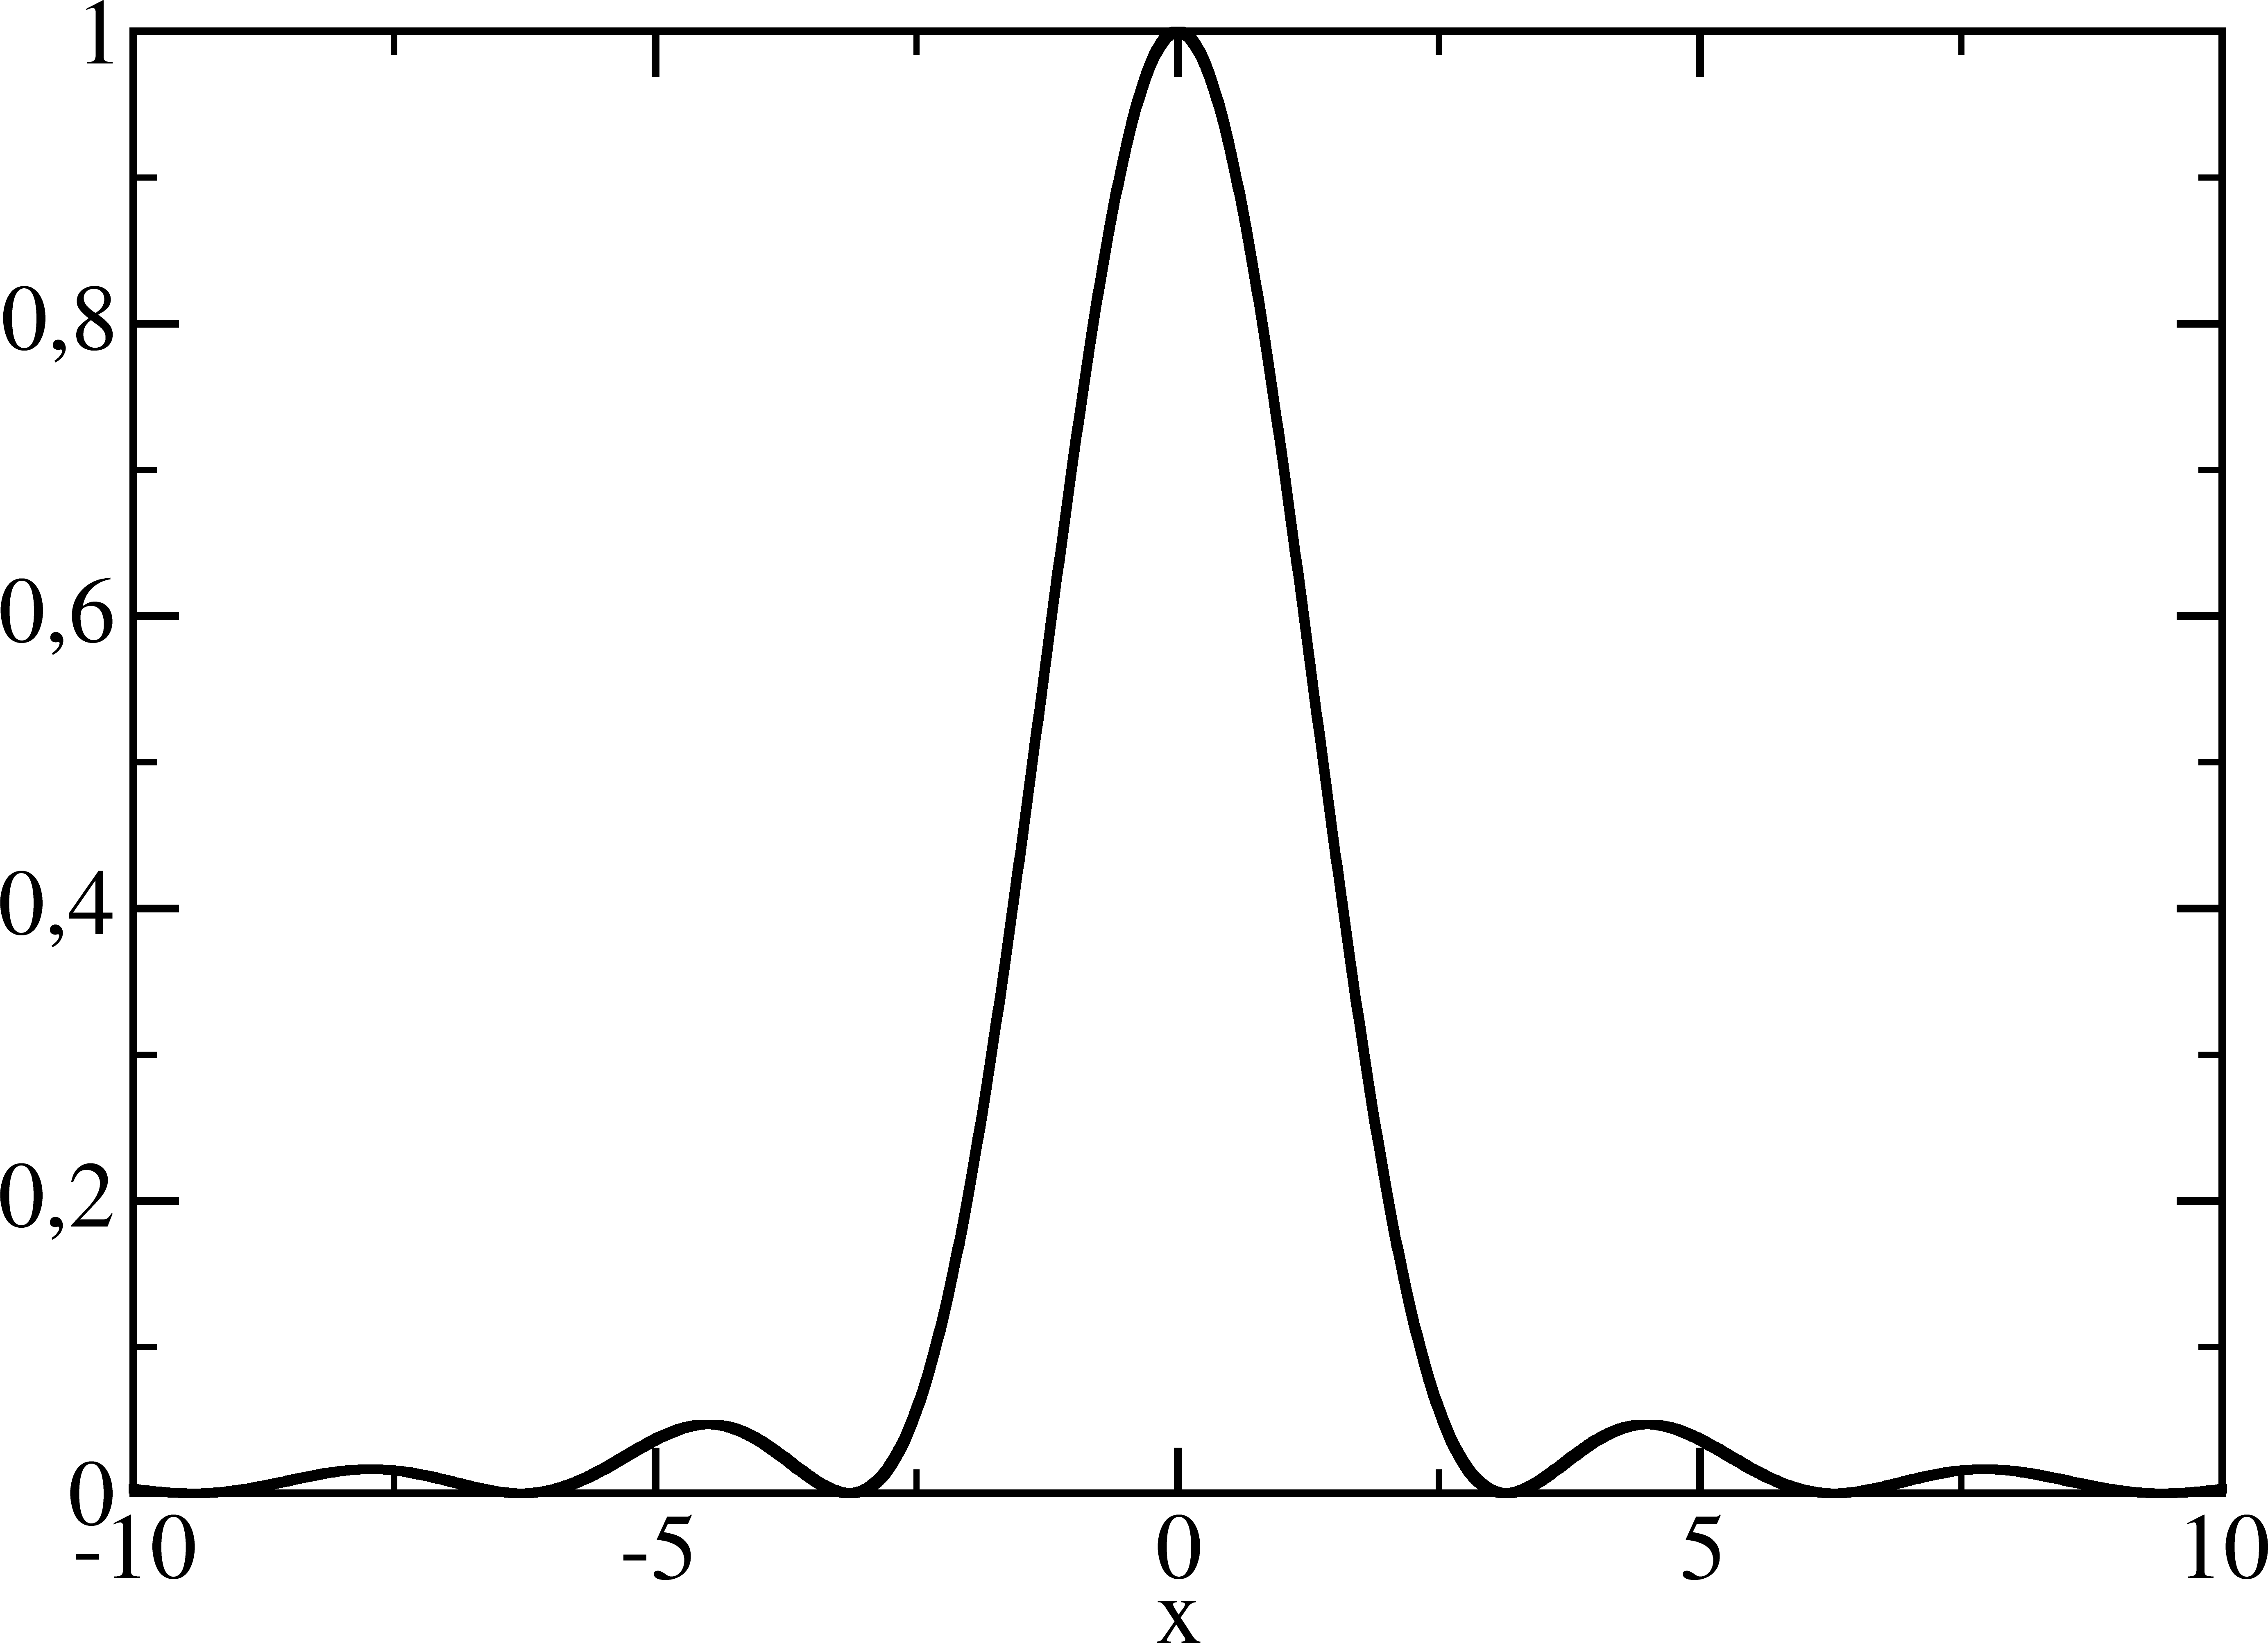
\includegraphics[width=8truecm]{slike/08_shg2.png}
\caption{Izkoristek pretvorbe v frekvenčno podvojeno valovanje je sorazmeren s funkcijo $(\sin(x)/x)^2$,
pri čemer je $x = \Delta k L/2$.}
\label{fig:shg2}
\end{figure}
Zaradi njega je na poti, ki je daljša od $\pi /\Delta k$, stopnja pretvorbe zelo majhna.

Poglejmo primer. Faktor $\Delta k$ je različen od nič zaradi odvisnosti
lomnih količnikov od frekvence. V KH$_{2}$PO$_{4}$ je 
redni lomni količnik pri 1000 nm 1,496, pri 500 nm pa 1,514. Vrednost, pri kateri
pade intenziteta frekvečno podvojenega valovanja na nič
$L_{c}=\pi /\Delta k$ je tako le okoli 30 mikrometrov. Na večjih dolžinah
postane stopnja pretvorbe zanemarljivo majhna.

Za visok izkoristek pretvorbe v frekvenčno podvojeno valovanje je torej 
pomembno, da se faze čim bolj ujemajo in da je $\Delta k = 0$. 
Takrat je vrednost faktorja $\sin(\Delta kL/2)/(\Delta kL/2)$ največja in izkoristek 
pretvorbe narašča sorazmerno s kvadratom dolžine
\beq
\frac{P_{2\omega}}{P_{\omega}}=
\frac{\omega^2 \chi_{ef}^2}{2 S n_{2\omega} n_\omega^2c_0^3\varepsilon_0} P_\omega L^2.
\eeq
Za uporabno pretvorbo v frekvenčno podvojeno valovanje je torej treba doseči 
fazno ujemanje valovnih vektorjev pri osnovni in podvojeni frekvenci. Kako to naredimo,
bomo spoznali v prihodnjem razdelku.

\begin{definition}
Pokazali smo, da intenziteta frekvenčno podvojenega valovanja narašča sorazmerno s
kvadratom debeline kristala. Takšna odvisnost velja le, če je intenziteta valovanja
pri podvojeni frekvenci bistveno manjša od intenzitete vpadnega valovanja, 
oziroma $A_3 \ll A_1, A_2$. Pokaži, da v nasprotnem primeru intenziteta frekvenčno
podvojenega valovanja $j_{2\omega}(L)$ narašča kot
\beq
j_{2\omega} (L) = j_0 \tanh^2 \left(\chi_{ef}\omega \sqrt{\frac{j_0}{2 n_3 n_1^2 c_0^3 \varepsilon_0}} L\right),
\eeq
pri čemer je $j_0$ vpadna intenziteta valovanja pri osnovni frekvenci. Namig: upoštevaj
ohranitev energije. 
\end{definition}

Povsem drugačno obnašanje dobimo v primeru, kadar pogoj ujemanja faz ni izpolnjen in 
 $\Delta k \neq 0$. Takrat dolžino kristala $L$ v izrazu~(\ref{8.11})
pokrajšamo in izkoristek pretvorbe z naraščajočim
$L$ sinusno niha med nič in neko največjo vrednostjo. Tak pojav lahko opazimo, če
imamo klinast vzorec, ki se mu debelina spreminja, ali pa če vzorec sučemo 
in na ta način spreminjamo razliko faz. Ta pojav, imenujemo ga Makerjeve 
oscilacije\footnote{P. D. Maker et al., Phys. Rev. Lett. 8, 21 (1962).}, 
uporabljamo za določanje nelinearne susceptibilnost kristalov.

% \begin{remark}
%  Odvisnosti stopnje pretvorbe od razlike valovnih vektorjev pri osnovni
% in podvojeni frekvenci je lahko razumeti s pomočjo slike~(\ref{fig:shg1}). Opazujmo
% prispevka k frekvenčno podvojenem valu, ki nastaneta eden na začetku kristala
% in drugi na koncu. Prispevek z začetka kristala zaradi disperzije na izhodni
% strani ni v fazi s prispevkom s konca. Pri dovolj veliki fazni razliki
% pride do destruktivne interference, ki zmanjšuje moč podvojene svetlobe.
% Razmere so podobne kot pri uklonu na široki reži, kjer prav tako seštevamo
% delna valovanja, ki se jim faza po reži linearno spreminja.
% \begin{figure}[h]
% \centering
% 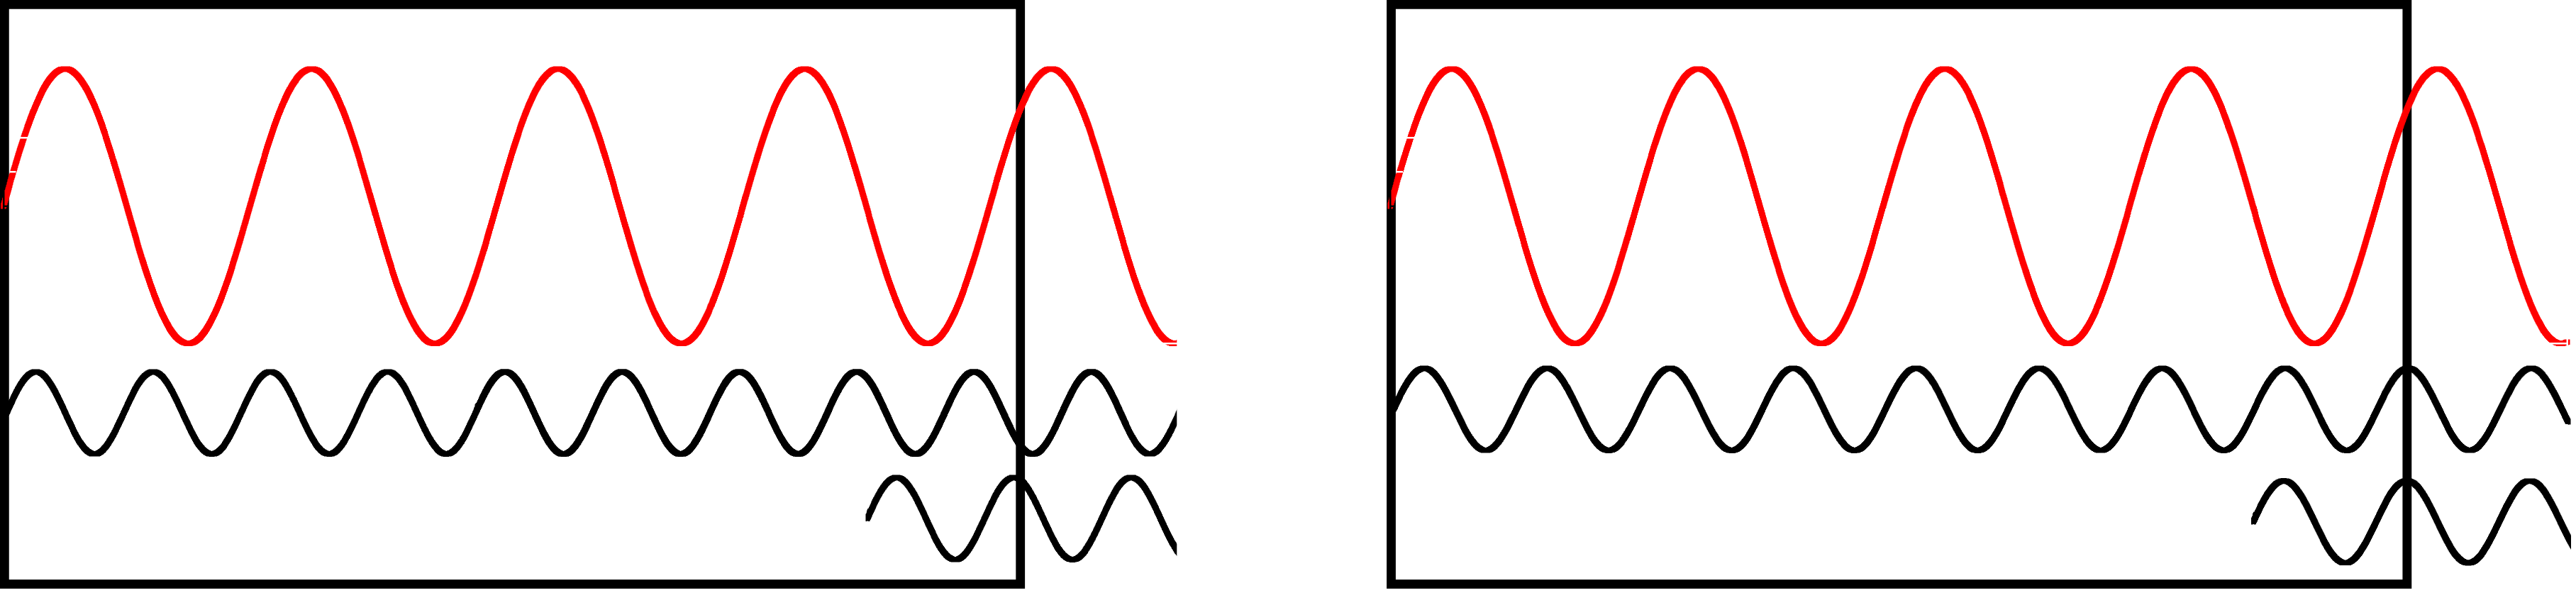
\includegraphics[width=10truecm]{slike/08_shg1.png}
% \caption{Levo: Neujemanje faz privede do destruktivne interference med valovi, ki nastajajo
% v različnih delih nelinearnega sredstva. Desno: V primeru, da se faze ujemajo, se valovanje 
% podvojeni frekvenci ojača.}
% \label{fig:shg1}
% \end{figure}
% \end{remark}

\subsection*{Ujemanje faz}
Poglejmo, kako lahko dosežemo ujemanje faz, ki je nujno za učinkovito optično
podvajanje frekvenc. Spomnimo se, da je pogoj za ujemanje faz 
\beq
\Delta k = k_3 - k_1 -k-2 = k_3^{2\omega} - k_1^{\omega} -k_2^\omega = 
\frac{2\omega}{c} n_3 - \frac{\omega}{c} n_1- \frac{\omega}{c} n_2 =0.
\eeq
Iz tega sledi pogoj za ujemanje faz
\boxeq{eq:dk0}{
n_1^\omega + n_2^\omega = n_3^{2\omega}.
}
Da lahko zadostimo gornjemu pogoju, izkoristimo dvojni lom v anizotropnih kristalih
(glej poglavje~\ref{chap:anizotropni}), pri čemer se zaradi enostavnosti omejimo le na optično 
enoosne kristale. Obravnavajmo samo kristale brez absorpcije in z normalno disperzijo, 
to pomeni, da oba lomna količnika naraščata s frekvenco.  

Za razumevanje je najbolj nazoren grafični prikaz (slika~\ref{fig:dk}). 
Podrobneje poglejmo primer s slike (a). Na njem so narisani lomni količniki za pozitivno
anizotropni ($n_e>n_o$) enoosni kristal pri enojni in dvojni
frekvenci v odvisnosti od kota glede na optično os. Rdeča barva nakazuje lomne količnike
pri vpadni frekvenci, modra pa pri podvojeni. Ekscentričnost elipse za 
izredni lomni količnik in frekvenčna disperzija sta zaradi večje nazornosti močno 
pretirani. Opazimo, da je pri nekem kotu $\vartheta$ med smerjo širjenja svetlobe in optično 
osjo redni lomni količnik pri dvojni frekvenci enak izrednemu količniku pri osnovni
frekvenci. Če torej izberemo izredno polarizacijo vpadnega vala (tako, ki leži
v ravnini optične osi in smeri širjenja), bo za podvojeni val z redno
polarizacijo (to je pravokotno na optično os) pri kotu
$\vartheta_m$ izpolnjen pogoj ujemanja faz~(enačba~\ref{eq:dk0}). Zapišimo to še z enačbo.

\begin{figure}[h]
\centering
\def\svgwidth{160truemm} 
\input{slike/08_phasematch.pdf_tex}
\caption{Štirje primeri, pri katerih je izpolnjen pogoj za ujemanje faz. 
(a) Ujemanje faz prvega reda za pozitivno anizotropno snov, (b)
ujemanje faz prvega reda za negativno anizotropno snov ter 
ujemanje faz drugega reda za pozitivno (c) in negativno (d) anizotropno snov.}
\label{fig:dk}
\end{figure}

Lomni količnik za redni val pri podvojeni frekvenci mora biti enak lomnemu 
količniku za izredni val pri osnovni frekvenci. Pri tem je lomni količnik
za izredni val odvisen od kota
\begin{equation}
\frac{1}{(n_o^{2\omega})^2} = \frac{1}{(n^{\omega}(\vartheta))^2}=
\frac{\cos^{2}\vartheta}{(n_{o}^{\omega})^2}+\frac{\sin^{2}\vartheta}{(n_{e}^{\omega})^2}.
\label{8.12}
\end{equation}
Tako dobimo 
\begin{equation}
\cos^{2}\vartheta_m=\frac{(n_o^{2\omega})^{-2}-(n_{e}^{\omega})^{-2}}
{(n_{o}^{\omega})^{-2}-(n_{e}^{\omega})^{-2}}.
\label{8.13}
\end{equation}
\begin{definition}
Pokaži, da v primeru negativne anizotropije pogoj za ujemanje faz zapišemo kot
\beq
\cos^{2}\vartheta_m=\frac{(n_o^{\omega})^{-2}-(n_{e}^{2\omega})^{-2}}
{(n_{o}^{2\omega})^{-2}-(n_{e}^{2\omega})^{-2}}.
\label{8.13a}
\eeq
\end{definition}

S slike~(\ref{fig:dk} c in d) lahko razberemo, da obstoja še en primer, pri 
katerem je izpolnjen pogoj za ujemanje faz. To je primer, pri katerem sta v vpadnem
valu prisotni obe polarizaciji, redna in izredna, podvojeni val pa
je spet redni. Tedaj mora biti za ujemanje faz redni lomni količnik
pri dvojni frekvenci enak povprečju rednega in izrednega lomnega količnika
pri osnovni frekvenci. Za praktično uporabo je ta izbira, kadar obstoja,
celo ugodnejša, ker je pri njej kot ujemanja faz bliže $\pi/2$. 
Ujemanje faz je zato manj občutljivo na majhna odstopanja v kotu ali na temperaturne
spremembe lomnih količnikov. Račun kota $\vartheta_m$ za ta primer je
bolj zahteven, saj je treba rešiti enačbo četrte stopnje.

\subsection*{Efektivna susceptibilnost}
Na moč podvojenega snopa poleg faznega faktorja vpliva tudi efektivna 
susceptibilnost $\chi_{ef}$, ki jo moramo izračunati za vsak primer posebej. 
V optično enoosnem kristalu
je kriterij ujemanja faz izpolnjen na stožcu okoli optične osi, pri čemer je stožec določen 
z izračunanim kotom $\vartheta_m$ (enačbi~\ref{8.13} in \ref{8.13a}). 
Drugi kot, ki določa smer širjenja v ravnini, ki je pravokotna na optično os, pa 
izberemo tako, da izkoristimo največje komponente nelinearne 
susceptibilnosti. 

Oglejmo si kot primer spet KH$_{2}$PO$_{4}$, ki je negativno anizotropen 
z vrednostmi $n_o^{\omega} = 1,4942$, 
$n_e^{\omega} = 1,4603$, $n_o^{2\omega} = 1,5129$ in $n_e^{2\omega} = 1,4709$
(slika~\ref{fig:dk}~b). Valovna dolžina osnovnega snopa naj bo 1064~nm. 
Po podatkih, navedenih zgoraj, dobimo po enačbi~(\ref{8.13a}) za kot ujemanja faz 
$\vartheta_m = 41,25^\circ$. Nelinearna susceptibilnost ima v tetragonalni
simetriji $\bar{4}2m$ od nič različne komponente $\chi_\textrm{xyz}$, 
$\chi_\textrm{zxy}$ in $\chi_\textrm{yzx}$ (glej tabelo~\ref{table:chi}). 
Zaradi poenostavitve privzamimo, da so njihove vrednosti enake. 
Smer širjenja osnovnega in podvojenega vala naj bo (slika \ref{fig:chi})
\begin{equation}
\mathbf{s}=(\cos\varphi\sin\vartheta_m,\sin\varphi\sin\vartheta_m,\cos\vartheta_m),
\label{8.14}
\end{equation}
kjer je $\varphi$ kot med osjo $x$ in projekcijo $\mathbf{s}$ na ravnino
$xy$, ki ga je treba še določiti. Poiščemo vrednost kota $\varphi$, pri katerem je 
moč frekvenčno podvojenega valovanja največja.
\begin{figure}[h]
\centering
\def\svgwidth{70truemm} 
\input{slike/08_chi.pdf_tex}
\caption{K izračunu efektivne susceptibilnosti. Rdeč vektror označuje
polarizacijo vhodnega vala, moder pa polarizacijo frekvenčno podvojenega vala.}
\label{fig:chi}
\end{figure}
Iz pogoja za ujemanje faz vidimo, da mora biti vpadna svetloba redno polarizirana, 
izhodna frekvenčno podvojena pa izredno polarizirana. Redna polarizacija je pravokotna na 
os $z$ (optično os) in hkrati pravokotna na smer vektorja $\mathbf{s}$. Zapišemo jo kot
\begin{equation}
\mathbf{e}_o=(\sin\varphi,-\cos\varphi,0),
\label{8.15}
\end{equation}
izredno polarizacijo pa kot
\begin{equation}
\mathbf{e}_e=(-\cos \varphi \cos \vartheta_m,-\sin \varphi \cos \vartheta_m ,\sin \vartheta_m).
\label{8.15a}
\end{equation}
Spomnimo se, da efektivno susceptibilnost izračunamo kot
\beq
\chi_{ef} = \sum_{ijk} \chi_{ijk} e_{ei} e_{oj} e_{ok}.
\eeq
Krajši račun pokaže, da je zaradi oblike tenzorja nelinearne susceptibilnosti v izbranem 
primeru od nič različna le $z$ komponenta nelinearne polarizacije. Dobimo
\beq
\chi_{ef} = \chi_{\textrm{zxy}} e_{ez} e_{ox} e_{oy} + \chi_{\textrm{zyx}} e_{ez} e_{oy} e_{ox}
\eeq
in
\begin{equation}
P_{\textrm{z}}^{2\omega}=- 2\varepsilon_0\, \chi_{\textrm{zxy}}E_{0}^2\cos\varphi\sin\varphi
\sin\vartheta_m = - \varepsilon_0\, \chi_{\textrm{zxy}}E_{0}^2\sin(2\varphi) \sin\vartheta_m.
\label{8.151}
\end{equation}
Nelinearna polarizacija je v tem primeru največja, kadar je $\varphi=\pi/4$.
Največji efektivni koeficient $\chi_{ef}$, ki nastopa v izrazih za amplitudo in 
moč podvojene svetlobe (enačbi~\ref{8.10} in \ref{8.11}), je torej v izbranem primeru 
\begin{equation}
\chi_{ef}= 
\sin\vartheta_m \chi_{\textrm{zxy}} \approx 0,66\, \chi_{\textrm{zxy}} \approx 0,66~\mathrm{pm/V}.
\label{8.16}
\end{equation}

\begin{definition}
Izračunaj efektivno nelinearno susceptibilnost za frekvenčno podvajanje svetlobe z valovno
dolžino 10~$\mu$m v kristalu telurja s simetrijsko grupo 32 (glej tabelo~\ref{table:chi}). 
Lomni količniki: $n_o^{\omega} = 4,7969$, 
$n_e^{\omega} = 6,2455$, $n_o^{2\omega} = 4,8657$ in $n_e^{2\omega} = 6,3152$.
\end{definition}

\section{Frekvenčno podvajanje Gaussovih snopov}

Doslej smo vpadni in frekvenčno podvojeni snop obravnavali kot ravni valovanji,
ki sta bili razsežni v prečni smeri. Izračunali smo, da v primeru ujemanja faz ($\Delta k=0$)
moč frekvenčno podvojene svetlobe narašča s kvadratom dolžine poti po nelinearnem
sredstvu. Pretvorba v frekvenčno podvojeno svetlobo je po enačbi~(\ref{8.11}) tem
učinkovitejša, čim večja je gostota svetlobnega toka pri osnovni frekvenci.
Zato v praksi vpadno svetlobo vselej fokusiramo.  

Poglejmo, kako se enačbe spremenijo, če je vpadni snop pri osnovni 
frekvenci Gaussove oblike. Rezultat lahko ocenimo, če vzamemo, da je
efektivna dolžina za pretvorbo $L$ kar dolžina grla; za njim se
gostota toka zmanjšuje, s tem pa tudi pretvorba v podvojeni snop.
Dolžina grla je 
\beq
L=2z_{0}=\frac{2n \pi w_{0}^{2}}{\lambda} = \frac{n w_0^2 \omega}{c_0}.
\label{SHGG}
\eeq
Tako je presek vpadnega snopa
\beq
S=\pi w_{0}^{2} = \frac{\pi c_0 L}{n \omega.}
\eeq
Daljše ko je grlo, večji je presek snopa in zato manjša intenziteta svetlobe. 
Vstavimo $S$ v enačbo~(\ref{8.11}), upoštevamo ujemanje faz in dobimo 
\begin{equation}
\frac{P_{2\omega}}{P_{\omega}}=
\frac{\omega^3 \chi_{ef}^2}{2 \pi n_{2\omega} n_\omega c_0^4\varepsilon_0} P_\omega\, L.
\label{8.17}
\end{equation}
Ob optimalnem fokusiranju je torej izkoristek pretvorbe sorazmeren z 
dolžino kristala in ne z njenim kvadratom.

\begin{definition}
Imamo 1~cm dolg kristal KH$_{2}$PO$_{4}$. Valovna dolžina vpadne svetlobe 
je 1,06~$\mu$m, vhodna moč $P_\omega = 10$~kW, efektivna nelinearna susceptibilnost
$\chi_{ef}=7\cdot10^{-13}~$m/V, $\Delta k=0$ in $n=1,5$. Pokaži, da je
faktor pretvorbe v frekvenčno podvojeno svetlobo okoli $20~\%$.

Da je dolžina grla $2z_{0}=1$~cm, mora biti polmer
grla okoli 40~$\mu$m. Gostota svetlobnega toka v kristalu je pri
tem $2\cdot10^{8}$~W/cm$^{2}$, kar je že blizu praga za poškodbe,
predvsem na vstopni ali izstopni površini. Zato je pri podvajanju frekvenc
zelo pomembna odpornost nelinearnega kristala proti poškodbam
zaradi velike gostote svetlobnega toka. To in možnost izpolnitve kriterija ujemanja 
faz sta poglavitna kriterija pri izbiri snovi za frekvenčno podvajanje. 
\end{definition}

\section{{*}Račun podvajanja Gaussovih snopov}

V prejšnjem razdelku smo na hitro grobo ocenili vpliv oblike Gaussovih snopov
na frekvečno podvajanje. Naredimo zdaj še natančejši izračun. Vrnimo se k valovni
enačbi~(\ref{8.3}) in spet imejmo vpadna snopa pri frekvencah
$\omega_{1}$ in $\omega_{2}$ in nastajajoč snop pri frekvenci
$\omega_{3}=\omega_{1}+\omega_{2}$.
Podobno kot prej naj ima vsako od polj obliko 
\beq
\mathbf{E}_{i}  = \frac{\mathbf{e}_{i}}{2}\left[\tilde{A}_{i}(r,z)\, 
e^{i(k_{i}z-\omega_{i}t)}+\tilde{A}_{i}^{*}(r,z)\, e^{-i(k_{i}z-\omega_{i}t)}\right],
\eeq
pri čemer je $A(r,z)$ zdaj funkcija tako vzdolžne kot tudi prečne koordinate. Privzeli
bomo, da se vzdolž $z$ le počasi spreminja.
Zaradi poenostavljenega zapisa vpeljimo novo spremenljivko 
\beq
\psi_i = \sqrt{\frac{n_i}{\omega_i}}\tilde{A}_i.
\eeq
Tako dobimo nastavek za električno poljsko jakost
\begin{equation}
\mathbf{E}_{i}=\frac{\mathbf{e}_{i}}{2}\sqrt{\frac{\omega_{i}}{n_{i}}}\psi_{i}(r,z)
e^{i(k_{i}z-\omega_{i}t)}+\mbox{ k. k.}
\label{8.18}
\end{equation}
Vstavimo nastavek~(\ref{8.18}) v valovno
enačbo~(\ref{8.3}) in ločimo na levi in desni člene z enako frekvenco.
Zaradi počasnega spreminjanja vzdolž smeri $z$ lahko zanemarimo tudi druge odvode 
$\psi$ po $z$. Tako dobimo sklopljen sistem obosnih enačb 
\begin{eqnarray}
\nabla_{\perp}^{2}\psi_{1}+2ik_{1}\psi_{1}^{\prime} & = & -
\frac{k_{1}}{2}\kappa\psi_{2}^{\ast}\psi_{3}e^{-i\Delta kz}\\
\nabla_{\perp}^{2}\psi_{2}+2ik_{2}\psi_{2}^{\prime} & = & -
\frac{k_{2}}{2}\kappa\psi_{1}^{\ast}\psi_{3}e^{-i\Delta kz}\\
\nabla_{\perp}^{2}\psi_{3}+2ik_{3}\psi_{3}^{\prime} & =
& - \frac{k_{3}}{2}\kappa\psi_{1}\psi_{2}e^{i\Delta kz}
\label{SHGGauss_3}
\end{eqnarray}
s pripadajočim sistemom konjugiranih enačb. Pri tem je 
\begin{equation}
\kappa=\frac{\chi_{ef}}{c_0} \sqrt{\frac{\omega_{1}\omega_{2}\omega_{3}}{n_{1}n_{2}n_{3}}}.
\label{8.20}
\end{equation}
S črtico smo označili odvajanje po $z$. Gornji sistem enačb je očitno
posplošitev sistema enačb~(\ref{eq:nlAz} do \ref{eq:nlA3}) za primer, ko je valovanje odvisno
tudi od prečne koordinate. Reševanje tega nelinearnega sistema parcialnih
diferencialnih enačb je seveda v splošnem zelo zapleteno.

Poglejmo le najenostavnejši primer frekvenčnega podvojevanja, ko je 
$\omega_{3}=2\omega_{1}=2\omega$.
Vpadna snopa naj bosta enaka in Gaussove oblike~(enačba~\ref{eq:gaussov-snop}), 
njuna amplituda pa naj bo enaka $A_1$
\begin{equation}
\psi_{1} = \psi_2 = A_{1}\frac{1}{1+iz/z_1}
\exp\left(-\frac{r^{2}}{w_1^{2}(z)}+\frac{ik_1r^{2}}{2R_1(z)}\right).
\label{8.21}
\end{equation}
Privzemimo še, da je izpolnjen pogoj za ujemanje faz, $\Delta k=0$,
in da je $\psi_{3}$ dovolj majhen, da nam zmanjševanja $\psi_{1}$
ni treba upoštevati. Tudi za podvojeni snop privzemimo Gaussovo 
obliko, njegova amplituda $A_3$ pa naj le počasi narašča
\begin{equation}
\psi_{3}=A_{3}(z)\psi_{3H}(z,r)=A_{3}(z)\frac{1}{1+iz/z_{3}}
\exp\left(-\frac{r^{2}}{w_{3}^{2}(z)}+\frac{ik_{3}r^{2}}{2R_{3}(z)}\right),
\label{8.22}
\end{equation}
pri čemer $\psi_{3H}$ reši homogeno obosno valovno 
enačbo~(\ref{eq:obosna-valovna-enacba}). Ko izraza za $\psi_{1}$
in $\psi_{3}$ vstavimo v tretjo enačbo sistema sklopljenih enačb (\ref{SHGGauss_3}),
ostane na levi le člen oblike $2ik_{3}A_{3}^{\prime}(z)\psi_{3H}$. Tako dobimo pogoj
\begin{equation}
A_{3}^{\prime}(z)\frac{1}{1+iz/z_3}\exp\left(-\frac{r^{2}}{w_{3}^{2}(z)}+\frac{ik_{3}r^{2}}
{2R_{3}(z)}\right)=
\frac{i\kappa}{4}A_{1}^{2}\frac{1}{(1+iz/z_{1})^{2}}\exp\left(-\frac{2r^{2}}
{w_{1}^{2}(z)}+\frac{ik_{1}r^{2}}{R_{1}(z)}\right).
\label{8.23}
\end{equation}
Poiščimo rešitev te enačbe v obliki, za katero velja $w_{30}^{2}=w_{10}^{2}/2$. Tedaj je 
\beq
z_{3}=\frac{k_{3}w_{30}^{2}}{2}=\frac{2k_{1}w_{10}^{2}}{4}=z_{1}
\eeq
in je tudi $w_{3}^{2}(z)=w_{1}^{2}(z)/2$. Poleg tega je $R_{3}(z)=R_{1}(z)$
in lahko na obeh straneh pokrajšamo eksponentna faktorja. Ostane 
\begin{equation}
A_{3}^{\prime}(z)=\frac{i\kappa}{4}A_{1}^{2}\frac{1}{1+iz/z_1}.
\label{8.24}
\end{equation}
Gornjo enačbo seveda brez težav integriramo. Naj bo grlo vpadnega
snopa ravno na sredini nelinearnega sredstva, tako da integriramo
od $-L/2$ do $L/2$
\begin{eqnarray}
A_{3}(L) & = & \frac{i\kappa}{4}A_{1}^{2}\int_{-L/2}^{L/2}\frac{dz}{1+iz/z_1} = \nonumber \\
 & = & \frac{\kappa}{4}A_{1}^{2}z_{1}\ln\frac{1+i\frac{L}{2z_{1}}}{1-i\frac{L}{2z_{1}}}= \nonumber \\
 & = & \frac{\kappa}{2}A_{1}^{2}z_{1}\arctan\frac{L}{2z_{1}}\;.
\end{eqnarray}
Moč Gaussovega snopa je
\begin{equation}
P_{i}=\pi w_{i0}^{2} \frac{1}{2}c_0 n_i \epsilon_{0}E_{i0}^{2}=
\frac{\pi}{2}w_{i0}^{2}\varepsilon_0 c_0 \omega_{i} A_{i}^{2},
\label{8.26}
\end{equation}
tako da je izkoristek pri frekvenčnem podvajanju Gaussovega snopa 
\begin{equation}
\frac{P_{2\omega}}{P_{\omega}}=\frac{A_3^2}{A_1^2} = 
\frac{\chi_{ef}^2 \omega^3 P_\omega z_1}{2 \pi c_0^4 \varepsilon_0 n_1 n_3} 
\arctan^2 \left( \frac{L}{2z_1}\right)
= \frac{\chi_{ef}^2 \omega^3 P_\omega}{2 \pi c_0^4 \varepsilon_0 n_1 n_3} \frac{L}{2}
\arctan^2 \left( \frac{L}{2z_1}\right) \frac{1}{L/2z_1}.
\label{8.27}
\end{equation}
Funkcija $(\arctan^{2}x)/x$ zavzame največjo vrednost pri 0,64 pri $x =L/2z_1=1,39$.
Pri dani dolžini nelinearnega sredstva $L$ dobimo torej največji
izkoristek, kadar je $z_{1}=0,36\,L$, kar je malo manj kot smo dobili
s preprosto oceno $2z_{1}=L$ (enačba~\ref{SHGG}). Največji izkoristek
frekvenčnega podvojevanja Gaussovih snopov je tako
\begin{equation}
\frac{P_{2\omega}}{P_{\omega}}
= 0,32 \frac{\chi_{ef}^2 \omega^3 }{2 \pi c_0^4 \varepsilon_0 n_1 n_3} P_\omega L.
\label{8.28}
\end{equation}
To je malo manj od preproste ocene, ki smo jo naredili v prejšnjem razdelku (enačba~\ref{8.17}),
v obeh primerih pa izkoristek narašča linearno z dolžino kristala.

\section{Optično parametrično ojačevanje}
\index{Optično parametrično ojačevanje}
\index{Parametrično ojačevanje | see {Optično parametrično ojačevanje}}

Oglejmo si še en zelo uporaben primer mešanja treh valov, 
ki ga opisujejo enačbe (\ref{eq:nlAz}) do (\ref{eq:nlA3}). Gre za
optično parametrično ojačevanje, pri katerem nelinearne optične pojave
izkoristimo za ojačevanje optičnih signalov. Imejmo vhodni
signal pri frekvenci $\omega_{1}$ skupaj z močnim črpalnim valom
pri frekvenci $\omega_{3}>\omega_{1}$. Zaradi nelinearnosti se ojačuje
val pri $\omega_{1}$, obenem pa nastaja dodaten val pri razliki frekvenc
$\omega_{2}=\omega_{3}-\omega_{1}$. Temu procesu pravimo parametrično
ojačevanje. Podoben princip se uporablja tudi v mikrovalovni tehniki,
od koder je tudi ime.

Prepišimo najprej enčbe \ref{8.8} v nekoliko prikladnejšo obliko,
kot smo napravili že pri vpeljavi sistema \ref{8.17}. Naj bo 
\begin{equation}
A_{i}(z)=\sqrt{\frac{n_{i}}{\omega_{i}}}E_{i}(z)\hskip0.5cm\mbox{in}
\hskip0.5cm\kappa=d\sqrt{\frac{\mu_{0}}{\epsilon_{0}}}\;.\label{8.30}
\end{equation}
 S tem dobijo enačbe \ref{8.8} obliko 
\begin{eqnarray}
\frac{dA_{1}}{dz} & = & \frac{i\kappa}{2}A_{2}^{\ast}A_{3}e^{i\Delta kz}\nonumber \\
\frac{dA_{2}^{\ast}}{dz} & = & \frac{-i\kappa}{2}A_{3}^{\ast}A_{1}e^{-i\Delta kz}\nonumber \\
\frac{dA_{3}}{dz} & = & \frac{i\kappa}{2}A_{1}A_{2}e^{-i\Delta kz}
\end{eqnarray}
 Privzemimo, da je črpalni val vselej dosti močnejši od ostalih dveh,
$A_{3}>>A_{1}$, $A_{2}$ in da smo poskrbeli za ujemanje faz, $\Delta k=0$.
$A_{3}$ je tako približno konstanta. Označimo še $g=\kappa/2A_{3}$,
pa imamo 
\begin{eqnarray}
\frac{dA_{1}}{dz} & = & igA_{2}^{\ast}\nonumber \\
\frac{dA_{2}^{\ast}}{dz} & = & igA_{1}
\end{eqnarray}
 Z začetnima pogojema $A_{1}(0)=A_{10}$ in $A_{2}(0)=0$ dobimo iz
\ref{8.32} rešitev 
\begin{eqnarray}
A_{1}(z) & = & A_{10}chgz\nonumber \\
A_{2}(z) & = & iA_{10}shgz
\end{eqnarray}
 Pri $z>1/g$ oba vala rasteta približno eksponentno na račun črpalnega
vala. Proces parametričnega ojačevanja si lahko predstavljamo kot
pretvorbo enega fotona pri frekvenci $\omega_{3}$ v fotona pri $\omega_{1}$
in $\omega_{2}$.

Privzeli smo, da je $\Delta k=k_{3}-k_{1}-k_{2}=0$. Ta pogoj lahko
izpolnimo na enak način kot pri podvajanju frekvence, to je tako,
da v dvolomnem kristalu izberemo ustrezno smer glede na optično os
in ustrezne polarizacije, tako da velja $\omega_{3}n_{3}=\omega_{1}n_{1}+\omega_{2}n_{2}$,
kjer so $n_{i}$ lomni količniki za odgovarjajoče valove pri izbranih
polarizacijah. Lahko na primer vzamemo izredno polarizacijo za črpalni
val in redni polarizaciji za oba ojačevana valova, podobno kot pri
podvajanju frekvence. Tedaj mora veljati 
\begin{equation}
n_{i}^{\omega_{3}}=\left[\left(\frac{cos\vartheta_{m}}{n_{r}^{\omega_{3}}}\right)^{2}
+\left(\frac{sin\vartheta_{m}}{n_{i0}^{\omega_{3}}}\right)^{2}\right]^{-1/2}=
\frac{\omega_{1}}{\omega_{3}}n_{r}^{\omega_{1}}+\frac{\omega_{2}}{\omega_{3}}n_{r}^{\omega_{2}}\;.\label{8.34}
\end{equation}
 Možne so seveda tudi drugačne izbire polarizacij (Naloga). (Naloga:
Obravnavaj parametrično ojačevanja, kadar je$\Delta k\neq0$.)

\textit{Primer:} Naj bo nelinearno sredstvo LiNbO$_{3}$, v katerem
je $d=5\cdot10^{-23}$~As/V in $n=2,2$. Vzemimo $\nu_{1}\simeq\nu_{2}=3\cdot10^{14}$~Hz
($\lambda_{1}=1\,\mu$m) in gostoto moči črpalnega vala 5~MW/cm$^{2}$.
Tedaj dobimo $g=0,67$~cm$^{-1}$.

Gornji primer kaže, da ojačenje ni prav veliko, kljub dokaj močnemu
črpalnemu valu. Zato je parametrično ojačevanje zanimivo predvsem
znotraj optičnih resonatorjev, s čemer dobimo neke vrste laser - \textit{parametrični
oscilator}.


\section{Nelinearni pojavi 3. reda}

Doslej smo obravnavali najnižji red nelinearnosti, katerega glavni
učinek je mešanje treh frekvenc, na primer podvajanje frekvence ali
parametrično ojačevanje. Ti pojavi so možni le v kristalih brez centra
inverzije. Naslednji člen razvoja nelinearne polarizacije po električnem
polju obstaja v vsaki snovi. V njem nastopa polje v tretji potenci.
Če vsebuje vpadno polje le eno frekvenco, zaradi nelinearnosti tretjega
reda dobimo polarizacijo pri 3$\omega$ in $\omega$. Pri dveh vpadnih
frekvencah $\omega_{1}$ in $\omega_{2}$ so možne kombinacije $2\omega_{1}\pm\omega_{2}$
in $\omega_{1}\pm2\omega_{2}$, pri treh vpadnih frekvencah pa vse
možne vsote in razlike frekvenc. Možnosti je torej precej več kot
pri nelinearnosti drugega reda. Obravnava nastajanja valovanja pri
kombinaciji frekvenc je povsem analogna podvajanju frekvence in parametričnemu
ojačevanju. V enačbah za nastajanje novega valovanja ali ojačevanje
katerega od vpadnih snopov spet nastopi fazni faktor, ki vsebuje razliko
vseh valovnih vektorjev $\Delta{\bf k}$. Da bo nastajanje novega
valovanja znatno, mora biti $\Delta kL\simeq0$, spet mora biti torej
izpolnjen pogoj ujemanja faz. Ker sedaj nastopajo v splošnem štirje
valovni vektorji, je seveda tudi pri izbiri geometrije in polarizacij
za ujemanje faz precej več možnosti.

Če vsebuje vapdno valovanje le eno frekvenco, je v nelinearni polarizaciji
tudi komponenta pri tej frekvenci, kar je ena od bistvenih razlik
med nelinearnostjo drugega in tretjega reda. Nelinearne pojave pri
eni sami frekvenci v\textquotedbl{}asih imenujejo tudi degenerirano
mešanje štirih valov. Najpreprostejši tak učinek je odvisnost lomnega
količnika od intenzitete vpadne svetlobe.

Vzemimo v smeri osi $x$ polarizirano valovanje, ki vpada na nelinearno,
zaradi enostavnosti izotropno snov. Nelinearna polarizacija ima tudi
le komponento 
\begin{equation}
P_{1}^{NL}=\epsilon_{0}\chi_{1111}^{(3)}E^{3}\label{8.70}
\end{equation}
 Polje spet zapišimo kot vsoto dveh konjugirano-kompleksnih členov:
\begin{equation}
E=\frac{1}{2}(E_{1}e^{i(kz-\omega t)}+E_{1}^{*}e^{-i(kz-\omega t)})\label{8.71}
\end{equation}
 Del polarizacije pri $\omega$ dobimo tako, da v izrazu za $E^{3}$
vzamemo dvakrat nekonjugirani del, enkrat pa konjugiranega. Taki členi
so trije. Tako imamo 
\begin{equation}
P_{1}^{\omega}=\frac{3}{8}\epsilon_{0}\chi_{1111}^{\left(3\right)}|E_{1}|^{2}E_{1}\label{8.72}
\end{equation}
 Ta del polarizacije lahko prištejemo k linearnemu delu in s tem dobimo
lomni količnik, ki je odvisen od intenzitete: 
\begin{equation}
\epsilon_{0}(\epsilon-1)E_{1}+\frac{3}{8}\epsilon_{0}\chi_{1111}^{\left(3\right)}|E_{1}|^{2}=\epsilon_{0}[n(I)^{2}-1]E_{1}\label{8.73}
\end{equation}
 Lomni količnik zapišimo v obliki 
\begin{eqnarray}
n(I) & = & n_{0}+n_{2}|E_{1}|^{2}\text{, }\\
n_{2} & = & \frac{3}{8}\chi_{1111}^{\left(3\right)}\text{ .}\label{8.74}
\end{eqnarray}
 Pojavu, pri katerem je sprememba lomnega količnika sorazmerna s kvadratom
električnega polja, smo imenovali Kerrov pojav. Ker je sedaj spremembo
povzroča kar optično polje samo, govorimo tudi o optičnem Kerrovem
pojavu. Zanimivi posledici sta samozbiranje svetlobnega snopa in širjenje
solitonov po optičnih vlaknih, kar si bomo pogledali v naslednjih
razdelkih.

Tudi splošni primer degeneriranega štirivalovnega mešanja je pomemben,
kjer se valovanja razlikujejo po smereh valovnih vektorjev. Vodi do
pojava \textit{fazne konjugacije. }Pri njem dobimo valovanje z enako
valovno fronto kot eno od vpadnih valovanj, ki pa se širi v nasprotni
smeri od prvotnega valovanja. Fazna konjugacija ima nekaj zanimivih
uporab in jo bomo obravnavali v zadnjem razdelku poglavja.


\section{Samozbiranje}

Poglejmo si najprej pojav \textit{samozbiranja }ali\textit{\ }samofokusacije
(anlgeško self focusing). Osnovni Gaussov snop naj vpada na sredstvo,
v katerem je lomni količnik odvisen od intenzitete po enačbi \ref{8.74}.
Optična Kerrova konstanta $n_{2\text{ }}$je običajno pozitivna. Tedaj
je lomni količnik v sredini snopa večji od nemotenega količnika na
robu. V osi snopa se optična pod podaljša in valovna fronta začne
v osi zaostajati glede na rob snopa. Če je zaostajanje dovolj veliko,
lahko krivinski radij valovne fronte postane negativen in snop se
ne širi, temveč oži (Slika\ref{sl8.10}). Samozbiranje je pri dovolj
veliki moči snopa tolikšno, da pride do katastrofične zožitve snopa
in s tem do tolikšnega povečanja gostote svetlobnega toka, da nastanejo
poškodbe v snovi.

Zaradi običajnega uklona se snop širi, pojav samozbiranja pa ima nasprotni
učinek. Zato je pri primerni moči snopa možno, da se oba pojava po
velikosti izenačita in snop ima v snovi konstanten polmer, valovne
fronte pa so ravne. Snop samemu sebi ustvarja valovni vodnik, kjer
je v sredi lomni količnik večji kot na robu. Ocenimo, kolišna mora
biti moč v stacionarnem stanju.

Vzemimo, da je na izbranem mestu valovna fronta ravna. Lahko si mislimo,
da je tam grlo Gaussovega snopa. Brez samozbiranja bi bil na razdalji
dolžine grla $z_{0}$ po izrazih iz drugega poglavja krivinski radij
valovne fronte 
\begin{equation}
R(z_{0})=z_{0}[1+\left(\frac{z_{0}}{z_{0}}\right)^{2}]=2z_{0}\label{8.75}
\end{equation}
 V bližini osi lahko Gaussovo funkcijo, ki opisuje prečno odvisnost
amplitude poja v snopu, razvijemo po prečni koordinati $r$ do drugega
reda; po enačbi \ref{8.74} je odvisnost lomnega količnika približno
\begin{equation}
n(r)=n_{0}+E_{0}^{2}(1-2\frac{r^{2}}{w_{0}^{2}})n_{2}\text{ .}\label{8.76}
\end{equation}
 Razlika med lomnim količniko na osi in pri $w_{0}$ od osi je $\Delta n=2E_{0}^{2}n_{2}$.
Zaradi tega je razlika optičnih poti za žarek na osi in za $w_{0}$
od osi $\Delta nz_{0}$. Valovna fronta bi se ukrivila na krivinski
radij $-R$. Iz preproste geometrije velja zveza 
\begin{equation}
\Delta nz_{0}=R-R\sqrt{1-\frac{w_{0}^{2}}{R^{2}}}\simeq\frac{1}{2}\frac{w_{0}^{2}}{R}\label{8.77}
\end{equation}
 Da bo valovna fronta ostala ravna, morata biti krivinska radija v
enačbah \ref{8.75} in \ref{8.77} enaka; od tu sledi 
\begin{equation}
\Delta n=\frac{w_{0}^{2}}{4z_{0}^{2}}\label{8.78}
\end{equation}
 Amplitudo polja v osi izrazimo z mo\textquotedbl{}jo: $E_{0}^{2}=2P/(\pi\epsilon_{0}cw_{0}^{2})$,
pa dobimo za moč snopa s stacionarnim polmerom 
\begin{equation}
P_{s}=\pi\epsilon_{0}c\frac{w_{0}^{4}}{2n_{2}z_{0}^{2}}=\frac{\epsilon_{0}c\lambda^{2}}{4n_{2}}\label{8.79}
\end{equation}
 Zanimivo je, da kritična moč ni odvisna od začetnega polmera snopa.
Pri manjši moči se snop širi, čeprav nekoliko počasneje kot v sredstvu
s konstantnim lomnim količnikom, če pa je moč znatno večja, lahko
pride do katastrofičnega samozbiranja in porušitve snovi.

\textit{Primer. }V CS$_{2}$, ki je tekočina z razmeroma velikim optičnim
Kerrovim pojavom, je $n_{2}=10^{-20}$~(m/V)$^{2}$. Tedaj dobimo
po gornji formuli za kritično moč vrednost 
\[
P_{s}=10^{4}\text{W.}
\]


Za podrobnejši račun moramo zapisati valovno enačbo v obosnem približku.
Začnimo spet s krajevnim delom valovne enačbe za monokromatsko valovanje
v skalarnem približku 
\begin{equation}
\nabla^{2}E+n^{2}\frac{\omega^{2}}{c^{2}}E=0\label{8.80}
\end{equation}
 Kot v drugem poglavju zapišimi polje v obliki počasi spreminjajoče
se amplitude in faznega faktorja: 
\begin{equation}
E=\psi(r,z)e^{ik_{0}z}\label{8.81}
\end{equation}
 kjer je $k_{0}=n_{0}\omega/c$ valovno število brez nelinearnosti.
$\psi(r,z)$ se v smeri osi $z$ le počasi spreminja, zato drugi odvod
po $z$ zanemarimo in dobimo 
\begin{equation}
\nabla_{\bot}^{2}\psi+\frac{\omega^{2}}{c^{2}}(n^{2}-n_{0}^{2})\psi+2ik_{0}\frac{\partial\psi}{\partial z}=0\label{8.82}
\end{equation}
 Upoštevajmo odvisnost lomnega količnika od intenzitete, pri čemer
zanemarimo člen z $n_{2}^{2}$, ker je gotovo majhen: 
\begin{equation}
\nabla_{\bot}^{2}\psi+2k_{0}^{2}\frac{n_{2}}{n_{0}}|\psi|^{2}\psi+2ik_{0}\frac{\partial\psi}{\partial z}=0\label{8.83}
\end{equation}
 Preden se lotimo reševanja gornje enačbe, jo še nekoliko polepšajmo.
Vpeljimo 
\begin{equation}
\kappa=2k_{0}^{2}\frac{n_{2}}{n_{0}}
\end{equation}
 in novo spremenljivko vzdolž osi $z$
\begin{equation}
\zeta=\frac{z}{2k_{0}}
\end{equation}
 S tem preide enačba \ref{8.83} v standardno oblikonelinearne Schrodingerjeve
enačbe 
\begin{equation}
i\frac{\partial\psi}{\partial\zeta}+\nabla_{\bot}^{2}\psi+\kappa\left|\psi\right|^{2}\psi=0\text{ .}\label{8.84}
\end{equation}


V treh dimenzijah je reševanje enačbe \ref{8.84} težavno in analitične
rešitve niso znane. V dveh dimenzijah pa stacionarno rešitev znamo
poiskati. Ker nam bo koristila tudi nekoliko kasneje pri računu širjenja
solitonov po optičnih vlaknih, si jo je vredno ogledati.

Stacionarni rešitvi se vzdolž $\zeta$ lahko spreminja le faza, zato
rešitev iščimo v obliki 
\begin{equation}
\psi=e^{i\eta^{2}\zeta}\, u(x)\label{8.87}
\end{equation}
 kjer je $\eta$ poljubna konstanta, katere pomen bomo videli kasneje.
Iz enačbe \ref{8.84} sledi za funkcijo $u(x)$, ki naj bo realna,
\begin{equation}
\frac{d^{2}u}{dx^{2}}=\frac{1}{2}\eta^{2}u-\kappa u^{3}
\end{equation}
 Z množenjem obeh strani z $u^{\prime}$ lahko enačbo enkrat integriramo
\begin{equation}
\left(\frac{du}{dx}\right)^{2}+C=\eta^{2}u^{2}-\frac{1}{2}\kappa u^{4}
\end{equation}
 Naj bo integracijska konstanta $C$ kar 0. Ločimo spremenljvki in
dobimo 
\begin{equation}
\int_{1}^{u}\frac{du}{u\sqrt{\eta^{2}-\frac{1}{2}\kappa u^{2}}}=x-x_{0}\label{8.85}
\end{equation}
 kjer smo novo integracijsko konstanto zapisali tako, da je pri $x=x_{0}$
vrednost $u=1$. Integral brez tezžav izračunamo: 
\begin{equation}
\ln\left(\sqrt{\frac{\kappa}{2}}\frac{u}{\eta+\sqrt{\eta^{2}-\kappa u^{2}/2}}\right)=x-x_{0}
\end{equation}
 Izarazimo iskano funkcijo: 
\begin{equation}
u=\sqrt{\frac{\kappa}{2}}\eta\frac{2}{e^{\eta(x-x_{0})}+e^{-\eta(x-x_{0})}}=\sqrt{\frac{\kappa}{2}\,}\eta\,\frac{1}{\text{ch}\eta(x-x_{0})}\label{8.86}
\end{equation}
 tako da je po enačbi \ref{8.87} 
\begin{equation}
\psi(x,z)=\sqrt{\frac{\kappa}{2}}\,\eta\,\frac{e^{i\eta^{2}\zeta}}{\text{ch}\eta(x-x_{0})}\label{8.88}
\end{equation}
 Vidimo, da predstavlja $1/\eta$ mero za polmer snopa, $x_{0}$ pa
je le prečni premik snopa, ki ga lahko brey škode postavimo 0. Tako
je polje stacionarnega snopa 
\begin{equation}
E_{s}(x,z)=\sqrt{\frac{\kappa}{2}\,}\frac{\eta}{\text{ch}\eta(x-x_{0})}\,\exp[ik_{0}z(1+\frac{\eta^{2}}{2k_{0}^{2}})]\label{8.89}
\end{equation}
 Od parametra $\eta$ je torej odvisna tudi konstanta širjenja in
s tem fazna hitrost. Ta je tem manjša, čim manjši je polmer snopa:
\begin{equation}
v_{f}=\frac{c}{n_{0}(1+\frac{\eta^{2}}{2k_{0}^{2}})}
\end{equation}


Moč dvodimenzionalnega snopa \ref{8.89} je sorazmerna z integralom
kvadrata polja po $x.$ Integriramo brez težav in dobimo 
\begin{equation}
\int|E_{s}|^{2}dx=\frac{2}{\kappa}\,\eta^{2}\int_{-\infty}^{\infty}\frac{dx}{\text{ch}^{2}\eta x}=\frac{4\eta}{\kappa}
\end{equation}
 Moč stacionarnega snopa v dveh dimenzijah je je obratno sorazmerna
s širino snopa $1/\eta$. Zato obstoja pri poljubni moči stacionarna
širina. To je bistvena razlika med dvo- in tridimenzionalnim primerom,
kjer se snop z nadkritično močjo krči v singularnost.


\section{Optični solitoni}

V prejšnjem razdelkusmo ugotovili, da pojav samozbiranja svetlobnega
snopa lahko ravno kompenzira širjenje zaradi uklona, tako da ima pri
ustrezni moči snop povsod konstnatno širino in obliko. Povsem analogen
pojav imamo tudi v časovni domeni. Sunek svetlob, ki se širi po snovi
s frekvenčno siperzijo lomnega količnika, se podaljšuje, kot smo ugotovili
v poglavju o optičnih vlaknih. Ob primernih pogojih lahko odvisnost
lomnega količnika od intenzitete ravno kompenzira disperzijo in sunek
ohranja obliko. Sunkom svetlobe, ki potujejo po sredstvu brez spremembe
oblike, pravimo tudi \textit{optični solitoni}. Posebej so pomembni
v optičnih vlaknih, kjer je disperzija izrazita in bi se je radi za
učinkovit prenos informacije čim bolj iznebili.

Poijav optičnih solitonov ni težko razložiti. V vrhu svetlobenga sunka
je pri $n_{2}>0$ lomni količnik največji, zato je na dani geometrijski
razdalji optična faza $k_{0}nz$ največja. Ker faza vzdolž sunka ni
več povsod enaka, se od začetka do konca sunka spreminja tudi frekvenca,
ki je odvod faze, in sicer je v sprednejm delu sunka nižja , v zadnjem
pa višja. Če je disperzija lomnega količnika taka, da grupna hitrost
narašča s frekvenco, bo zadnji del sunka dohiteval sprednjega. Ta
učinek nelinearnosti lahko ravno kompenzira širjenje sunka zaradi
disperzije.

Računsko obravnavajmo primer širjenja solitona po enorodnem optičnem
vlaknu. Spomnimo se (en. \ref{?.??}), da se zaradi spremembme lomnega
količnika vlakna spremeni valovno število 
\begin{equation}
\delta\beta=\frac{\omega^{2}}{c^{2}\beta}\,\frac{\int n\,\delta n\,|u|^{2}dS}{\int|u|^{2}dS}\label{8.90}
\end{equation}
 kjer $u(r)$ opisuje prečno obliko valovanja v vlaknu. Valovno število
je v vlaknu funkcija frekvence. Kot v razdelku ???? ga razvijmo okoli
centralne frekvence in dodajmo še prispevek \ref{8.90}: 
\begin{equation}
\beta\left(\omega\right)=\beta\left(\omega_{0}\right)+\frac{d\beta}{d\omega}\,(\omega-\omega_{0})+\frac{1}{2}\frac{d^{2}\beta}{d\omega^{2}}(\omega-\omega_{0})^{2}+\frac{\omega^{2}}{c^{2}\beta}\,\frac{\int n\,\delta n\,|u|^{2}dS}{\int|u|^{2}dS}\label{8.91}
\end{equation}
 Svetlobni sunek, ki se širi po vlaknu, zapišimo, kot smo že vajeni,
v obliki počasi spreminjajoče se amplitudne funkcije in faznega faktorja
pri nosilni frekvenci: 
\begin{equation}
E\left(r,z,t\right)=A\left(z,t\right)\, u\left(r\right)\,\exp i\left[\beta\left(\omega_{0}\right)z-\omega_{0}t\right]\label{8.92}
\end{equation}
 V razdelku ???? smo s pomočjo razvoja \ref{8.91} in Foureirove transformacije
izpeljali diferencialno enačbo ??? za $A\left(z,t\right)$. Na isti
način moramo sedaj le dodati člen $\delta\beta$ iz en. \ref{8.90}:
\begin{equation}
(\frac{\partial}{\partial z}+\frac{1}{v_{g}}\frac{\partial}{\partial t})A=-\frac{i}{2}\frac{d^{2}\beta}{d\omega^{2}}\,\frac{\partial^{2}A}{\partial t^{2}}+i\kappa|A|^{2}A\label{8.93}
\end{equation}
 kjer je 
\begin{equation}
\kappa=\frac{\omega^{2}}{c^{2}\beta}\,\frac{\int n_{0}\, n_{2}\,|u|^{4}dS}{\int|u|^{2}dS}\label{8.94}
\end{equation}


Vpeljimo novo neodvisno spremenljivko 
\begin{equation}
\tau=t-\frac{z}{v_{g}}
\end{equation}
 s katero opišemo obliko sunka, kot ga vidi opazovalec, ki se giblje
z grupno hitrostjo skupaj s sunkom. Enačba \ref{8.93} dobi s tem
obliko 
\begin{equation}
i\,\frac{\partial A}{\partial z}-\frac{1}{2}\frac{d^{2}\beta}{d\omega^{2}}\,\frac{\partial^{2}A}{\partial\tau^{2}}+\kappa\left|A\right|^{2}A=0\label{8.95}
\end{equation}
 Ta enačba ima kot pri obravnavi samozbiranja svetlobnega snopa v
prejšnjem razdelku obliko nelinearne Schrodingerjeve enačbe \ref{8.84},
v kateri ima sedaj $\tau$ isto vlogo kot prej prečna koordinata $x$.
Rešitev s stacionarno dolžino sunka, ki ustreza rešitvi s konstantnim
premerom snopa v primeru samozbiranja, tako dobimo, kadar je $d^{2}\beta/d\omega^{2}<0$.
To pomeni, da grupna hitrost narašča s frekvenco, kar je v skladu
z razmislekom na začetku tega razdelka. Optični soliton v vlaknu ima
torej obliko 
\[
A\left(z,\tau\right)=\sqrt{\frac{2}{\kappa}}\frac{\eta}{{\rm ch}\left[\sqrt{2\left|\frac{d^{2}\beta}{d\omega^{2}}\right|^{-1}}\eta\tau\right]}\,\exp\left(i\eta^{2}z\right)
\]
 
\begin{equation}
A\left(z,t\right)=\sqrt{\frac{2}{\kappa}}\frac{\eta}{{\rm ch}\left[\sqrt{2\left|\frac{d^{2}\beta}{d\omega^{2}}\right|^{-1}}\frac{\eta}{v_{g}}\left(v_{g}t-z\right)\right]}\,\exp\left(i\eta^{2}z\right)\label{8.96}
\end{equation}
 Parameter $\eta$ je sorazmeren z energijo solitona. Ta potuje z
grupno hitrostjo in pri tem ohranja obliko. Analiza majhnih odmikov
od dobljene rešitve pokaže, da je soliton tudi stabilen ( Naloga).
Zaradi tega se zdi, da bilo solitone mogoče izrabiti v optičnih komunikacijskih
sistemih, kjer je potrebna velika gostota prenosa informacije na velike
razdalje. S tem bi se izognili težavam, ki jih pri linearnem prenosu
povzroča disperzija.


\section{Optična fazna konjugacija}

\textit{Fazna konjugacija} je zanimiv in danes tudi prektično pomemben
pojav, pri katerem dobimo iz danega novo valovanje, ki ima enake valovne
fronte in potuje v nasprotni smeri od prvotnega valovanja; novo valovanje
je tako, kot bi začetnemu obrnili predznak časa. Pojav je v ozki zvezi
s holografijo, kjer najprej zapišemo predmetni snop, ki ga kasneje
reproduciramo, pri fazni konugaciji pa zapis začetnega vala in njegova
reproducija potekata sočasno.

Napravimo poskus, ki ga kaže slika \ref{sl8.31}. Na nelinearen kristal
naj v nasprotnih smereh vpadata dva močna ravna črpalna vala z valovnima
vektorjema ${\bf k}_{1}$ in $-{\bf k}_{1}$. Poleg tega naj vpada
še tretji, signalni snop, ki ni nujno raven val. Signalni val interferira
s prvim črpalnim valom in s tem zaradi nelineranosti tretejga reda
povzroči modulacijo lomnega količnika, ki je skoraj periodična, če
je signalni val blizu ravnega vala. Na tej periodični modulaciji se
drugi črpalni val uklanja, pri čemer je uklonjeni val enake oblike
kot signalni, le potuje v nasprotni smeri, ker ima drugi črpalni val
nasprotno smer od prvega. Črpalna vala sta seveda enakovredna in ni
mogoče ločiti, s katerim je signalni val interferiral in kateri se
uklanja.

Pozoren bralec je ugotovil, da je gornja razlaga podobna razlagi holografije,
le da sta tam postopka zapisa interference predmetnega vala z refernčnim
in reprodukcije ločena.

Signalni val lahko zapišemo v obliki 
\begin{equation}
E_{3}=\mathrm{Re}\left[\psi\left(r\right)\, e^{i\left(kz-\omega t\right)}\right]\label{8.97}
\end{equation}
 Videli bomo, da je novonastali val 
\begin{equation}
E_{4}=\mathrm{Re}\left[\psi^{*}\left(r\right)\, e^{i\left(-kz-\omega t\right)}\right]\label{8.98}
\end{equation}
 Zaradi nasprotnega predznaka $k$ potuje v obratni smeri od signalnega
vala; poleg tega je še amplituda konjugirano kompleksna. To seveda
ne pliva na obliko valovnih front, te so popolnoma enake kot pri signalnem
valu. Zaradi lastnosti, da lahko novi val iz signalnega dobimo tako,
da krajevni del kompleksno konjugiramo, nastalemu valu pravimo fazno
konjugiran val.

Uporabna posledica fazne konjugacije je prikazana na sliki \ref{sl8.32}.
Naj na neko nerpavilno sredstvo z leve vpada Gaussov snop. Po prehodu
skozi sredstvo valovne fronte niso več gladke. Ta popačen snop v faznem
konjugatorju generira fazno konjugiran snop, ki potuje proti levi
in ima enako nepravilne valoven fronte kot vpadni val. Po prehodu
skozi nepravilno sredstvo se neravnosti valovne fronte kompenzirajo
in dobimo enake gladke valoven ploskeve Gaussovega snopa, kot smo
jih imeli na začetku. To lastnost popravljanja valovne fronte je mogoče
koristni uporabiti, na primer namesto enega zrcala v laserskem resonatorju.

Poglejmo podrobneje, kako v nelinearnem sredstvu nastane fazano konjugiran
val. Kot kaže slika \ref{sl8.31}, je celotno polje v nelienarnem
kristalu vsota štirih valov, dveh črpalnih, signalnega in odbitega:
\begin{equation}
E=\frac{1}{2}E_{1}e^{i{\bf k}_{1}\cdot{\bf r}}+\frac{1}{2}E_{2}e^{-i{\bf k}_{1}\cdot{\bf r}}+\frac{1}{2}E_{3}\left(z\right)e^{ikz}+\frac{1}{2}E_{4}\left(z\right)e^{-ikz}+{\rm k.k.}\label{8.99}
\end{equation}
 S k.k. smo spet označili konjugirano kompleksne člene. Ker so vsa
polje pri isti frekvenci, nam časovenga faktorja ni treba pisati.
Zaradi enostavnosti zapisa nelinearne polarizacije vzemimo, da so
vse polarizacije enake. Privzeli smo še, da sta črpalna vala $E_{1}$
in $E_{2}$ dosti močnejša od $E_{3}$ in $E_{4}$, tako da sta njuni
amplitudi konstantni, $E_{3}\left(z\right)$ in $E_{4}\left(z\right)$
pa se le počasi spreminjata.

Postavimo $E$ v časovno neodvisno valovno enačbo z nelinearno polarizacijo:
\begin{equation}
\nabla^{2}E+\epsilon\frac{\omega^{2}}{c^{2}}\, E=-\mu_{0}\omega^{2}P^{NL}\label{8.100}
\end{equation}
 Pri tem je $\epsilon\,\omega^{2}/c^{2}=k^{2}$. Ker obravnavamo le
polje pri osnovni frekvenci, nastopajo v nelinearni polarozaciji le
členi s to frekvenco. Vsebujejo še vedno različne kombinacije valovnih
vektorjev. K enačbi za $E_{4}$ prispevajo le tisti s krajevnim faznim
faktorjem $\exp(-ikz)$, to je 
\begin{equation}
P_{4}^{NL}=\epsilon_{0}\chi^{\left(3\right)}[E_{1}E_{2}E_{3}^{*}+(\left|E_{1}\right|^{2}+\left|E_{2}\right|^{2})E_{4}]\label{8.101}
\end{equation}
 Tu je $\chi^{\left(3\right)}$ efektivna nelinearna susceptibilnost
za izbrano polarizacijo vseh polj. Zanemarili smo člene, kjer $E_{3}$
in $E_{4}$ nastopata v višjih potencah, ker so majhni v primeri z
zapisanimi. Z upoštevanjem, da se $E\left(z\right)$ le počasi spreminja,
dobimo enako kot pri mešanju treh frekvenc 
\begin{equation}
\frac{dE_{4}}{dz}=i\frac{\omega}{nc}\,\chi^{\left(3\right)}\left[E_{1}E_{2}E_{3}^{*}+(\left|E_{1}\right|^{2}+\left|E_{2}\right|^{2})E_{4}\right]\label{8.102}
\end{equation}
 Drugi člen na desni že poznamo; opisuje odvisnost lomnega količnika
od intenzitete črpalnih valov, torej optični Kerrov pojav. Vpeljimo
nove amplitude 
\begin{equation}
A_{k}=E_{k\,}\exp\left[-i\frac{\omega}{nc}\left(\left|E_{1}\right|^{2}+\left|E_{2}\right|^{2}\right)z\right]\label{8.103}
\end{equation}
 ki se od prvotnih razlikujejo le po faznem faktorju. S tem se enačba
\ref{8.102} poenostavi: 
\begin{equation}
\frac{dA_{4}}{dz}=i\frac{\omega}{nc}\,\chi^{\left(3\right)}A_{1}A_{2}A_{3}^{*}\label{8.104}
\end{equation}
 Podobno dobimo 
\begin{equation}
\frac{dA_{3}^{*}}{dz}=i\frac{\omega}{nc}\,\chi^{\left(3\right)}A_{1}^{*}A_{2}^{*}A_{4}\label{8.105}
\end{equation}
 Z vpeljavo sklopitvene konstante 
\begin{equation}
\kappa=\frac{\omega}{nc}\,\chi^{\left(3\right)}\label{8.106}
\end{equation}
 se enačbi poenstavita: 
\[
\frac{dA_{4}}{dz}=i\kappa^{*}A_{3}^{*}
\]
 
\begin{equation}
\frac{dA_{3}^{*}}{dz}=i\kappa A_{4}\label{8.107}
\end{equation}


Bralcu priporočam, da si še enkrat ogleda korake, s katerimi smo zelo
težaven problem nelinearne valovne enačbe poenostavili na lineanren
sistem dveh preprostih sklopljenih enačb za amplitudi signalnega in
odbitega vala.

Splošni rešitvi sistema \ref{8.107} sta 
\begin{eqnarray}
A_{4}\left(z\right) & = & C_{1}\cos\left|\kappa\right|z+C_{2}\sin\left|\kappa\right|z\label{8.108}\\
A_{3}^{*}\left(z\right) & = & -i\frac{\left|\kappa\right|}{\kappa^{*}}\left(-C_{1}\sin\left|\kappa\right|z+C_{2}\cos\left|\kappa\right|z\right)\nonumber 
\end{eqnarray}
 Potrebujemo še robne pogoje za obe valovanji. Z leve, pri $z=0$,
poznamo $A_{3}^{*}\left(0\right)$, pri $z=L$ pa ne more biti odbitega
vala:$A_{4}\left(L\right)=0$. S tem lahko določimo konstanti $C_{1}$
in $C_{2}$: 
\begin{eqnarray}
A_{4}\left(z\right) & = & i\frac{\kappa^{*}}{\left|\kappa\right|}\frac{\sin\left|\kappa\right|\left(L-z\right)}{\cos\left|\kappa\right|L}A_{3}^{*}\left(0\right)\label{8.109}\\
A_{3}^{*}\left(z\right) & = & \frac{\cos\left|\kappa\right|\left(z-L\right)}{\cos\left|\kappa\right|L}A_{3}^{*}\left(0\right)\nonumber 
\end{eqnarray}
 Amplituda odbitega vala pri $z=0$ je 
\begin{equation}
A_{4}\left(0\right)=i\frac{\kappa^{*}}{\left|\kappa\right|}\tan\left|\kappa\right|L\; A_{3}^{*}\left(0\right)\label{8.110}
\end{equation}
 Odbiti val je sorazmeren s kompleksno konjugirano amplitudo vpadnega
vala in ima natnako nasproten valovni vektor, zato tudi ime fazno
konjugiran val. Ker je lahko $\tan\left|\kappa\right|L>1$, je možno
tudi ojačenje odbitega vala, ki gre seveda na račun moči črpalnih
valov.

Doslej smo predpostavili, da je signalni val raven. Če je njegova
amplituda odvisna še od prečne koordinate, ga lahko razvijemo po ravnih
valovih in velja za vsako komponento posebej en. \ref{8.110}. Odbite
komponente so sorazmerne s konjugiranimi komponentami signalnega vala
z nasprotnim valovnim vektorjem in dajo skupaj valovno fronto enake
oblike kot pri signalnem valu, le giblje se v nasprtni smeri, kot
smo opisali že na začetku razdelka.

V NOVO POGLAVJE
Poseben primer nelinearne susceptibilnosti $d_{ijk}$ smo pravzaprav
že srečali pri elektrooptičnem pojavu: elektrooptični tenzor $r_{ijk}$
opisuje isto lastnost snovi, le da smo tam zahtevali, da je eno polje
skoraj statično. Za $d_{ijk}$ velja, kot za vsak tenzor tretjega
ranga, da je lahko od nič različen le v snoveh brez centra inverzije.
V centrosimetričnih snoveh je prvi od nič različni nelinearni člen
tretjega reda.